%\documentclass[first,firstsupp,handout,compress,notes,navigation]{ETHclass} 
%\documentclass[first,firstsupp,handout,lastsupp]{ETHclass} 
\documentclass[first,firstsupp,lastsupp,handout,last,hyperref,table]{ETHclass} 
%\documentclass[first,firstsupp]{ETHclass}
\usepackage{etex}

\usepackage{adjustbox}
\usepackage{amsmath}
\usepackage{amssymb}
\usepackage{animate}
\usepackage{booktabs}
\usepackage{charter}
\usepackage{enumitem}
\usepackage{etoolbox}
\usepackage{ifthen}
\usepackage{longtable}
\usepackage{mathrsfs}
\usepackage{multicol}
\usepackage{pgf}
\usepackage{pgfplots}
\usepackage{pifont}
\usepackage{ragged2e}
\usepackage{standalone}
\usepackage[caption=false]{subfig}
\usepackage{tabularx}
\usepackage{tikz}
\usepackage{verbatim}
\usepackage{xcolor}
\usepackage{hyperref}

\pgfplotsset{compat=1.7}

\setbeamertemplate{navigation symbols}{}
\usetikzlibrary{arrows,decorations.pathreplacing,positioning,shapes,shadows}

%\usepackage[style=numeric-comp]{biblatex}

%\usepackage{lipsum}

%\usetikzlibrary{fit}
\usetikzlibrary{arrows}
\usetikzlibrary{trees}

% Options for beamer:
%
% 9,10,11,12,13,14,17pt  Fontsizes
% 
% compress: navigation bar becomes smaller
% t       : place contents of frames on top (alternative: b,c)
% handout : handoutversion
% notes   : show notes
% notes=onlyslideswithnotes
%
%hyperref={bookmarksopen,bookmarksnumbered} : Needed for menues in
%                                             acrobat. Also need
%                                             pdftex as option or 
%                                             compile with
% pdflatex '\PassOptionsToPackage{pdftex,bookmarksopen,bookmarksnumbered}{hyperref} \input{file}'

%\usepackage{beamerseminar}
%\usepackage[accumulated]{beamerseminar}
                                % remove ``accumulated'' option
                                % for original behaviour
%\usepackage{beamerbasenotes}
%\setbeamertemplate{note page}[plain] 
%\setbeameroption{notes on second screen}

%\setbeamertemplate{note page}[plain] 
\setbeamertemplate{note page}{\ \\[.3cm]
\textbf{\color{blue}Notes:}\\%[0.1cm]
{\footnotesize %\tiny
\insertnote}}
%\setbeameroption{notes on second screen}


%\setbeamertemplate{navigation symbols}{} % suppresses all navigation symbols:
 \setbeamertemplate{navigation symbols}[horizontal] % Organizes the navigation symbols horizontally.
% \setbeamertemplate{navigation symbols}[vertical] % Organizes the navigation symbols vertically.
% \setbeamertemplate{navigation symbols}[only frame symbol] % Shows only the navigational symbol for navigating frames.

\setlayoutscale{0.5}
\setparametertextfont{\scriptsize}
\setlabelfont{\scriptsize}

% \useoutertheme[subsection=false]{miniframes}
% \usepackage{etoolbox}
% \makeatletter
% \patchcmd{\slideentry}{\advance\beamer@xpos by1\relax}{}{}{}
% \def\beamer@subsectionentry#1#2#3#4#5{\advance\beamer@xpos by1\relax}%
% \makeatother

% \makeatletter
%     \newenvironment{withoutheadline}{
%        \setbeamertemplate{headline}{%
% \vspace{15pt}
% }
%     }{}
% \makeatother

\makeatletter
    \newenvironment{withoutheadline}{
         \setbeamertemplate{headline}{%
\vspace{35pt}
}
        %\def\beamer@entrycode{\vspace*{-1.5\headheight}}
    }{}
\makeatother

\newcommand{\Cross}{$\mathbin{\tikz [x=1.4ex,y=1.4ex,line width=.2ex, red] \draw (0,0) -- (1,1) (0,1) -- (1,0);}$}%

\newcommand{\Checkmark}{$\color{green}\checkmark$}

\setbeamerfont{subsection in toc}{size=\tiny}

\makeatletter
\patchcmd{\beamer@sectionintoc}
  {\vfill}
  {\vskip1.5\itemsep}
  {}
  {}
\makeatother  

\setbeamertemplate{frametitle continuation}{}

\setbeamertemplate{bibliography entry title}{}
\setbeamertemplate{bibliography entry author}{}
\setbeamertemplate{bibliography entry location}{}
\setbeamertemplate{bibliography entry note}{}

\setbeamercolor*{bibliography entry title}{fg=black}
\setbeamercolor*{bibliography entry author}{fg=black}
\setbeamercolor*{bibliography entry location}{fg=black}
\setbeamercolor*{bibliography entry note}{fg=black}
% and kill the abominable icon
%\setbeamertemplate{bibliography item}{\color{forestgreen}$\blacktriangleright$}
\setbeamertemplate{bibliography item}{\insertbiblabel}
%\setbeamertemplate{bibliography item}{\theenumiv}

\newcommand{\highlightred}[1]{%
  \colorbox{red!50}{$\displaystyle#1$}}
  
\newcommand{\highlightyellow}[1]{%
  \colorbox{yellow!50}{$\displaystyle#1$}}
  
\newcommand{\highlightgreen}[1]{%
  \colorbox{green!50}{$\displaystyle#1$}}

\AtBeginSection[]{
  \begin{frame}
  \vfill
  \centering
  \begin{beamercolorbox}[sep=8pt,center,shadow=true,rounded=true]{title}
    \usebeamerfont{frametitle}
\includegraphics[width=2ex]{freccia_trasparente_verde_foresta.png}\hspace{.5ex}~{\LARGE \textsc{\bfseries \insertsectionhead}}\par%
  \end{beamercolorbox}
  \vfill
  \end{frame}
}

\hyphenpenalty=5000
\tolerance=1000

\graphicspath{{figures/}}

\newenvironment{system}{\left\lbrace\begin{array}{@{}l@{}}}{\end{array}\right.}

\newenvironment{subsystem}{\left\lgroup\begin{array}{@{}l@{}}}{\end{array}\right.}

\defbeamertemplate*{title page}{customized}[1][]
{
\usebeamerfont{subtitle}
\usebeamercolor[fg]{subtitle}

\vspace{-1.75cm}

{\center
 \usebeamerfont{title}{\inserttitle}\par
}
\vspace{-.25cm}
{\flushleft
 \usebeamerfont{subtitle}{\small \insertsubtitle} \par
}

%\vspace{-.5cm}

{\center
\setbeamercolor{author}{bg=white,fg=Red}
\usebeamerfont{author}{\footnotesize \insertauthor} \par}

\vspace{-.2cm}

{\center
\usebeamerfont{institute}{\tiny \insertinstitute}\par }

\vspace{.2cm}

{\center
\usebeamerfont{date}{\scriptsize \insertdate} \par }

\vspace{0.2in}
}


\begin{document}
\setbeamertemplate{caption}{\raggedright\insertcaption\par}

\title{\textsc{Update 2017-06-23}}
\author{ L. Di Stasio$^{1,2}$, Z. Ayadi$^{1}$, J. Varna$^{2}$}
%\institute{ Science et Ing\'enierie des Mat\'eriaux et M\'etallurgie (SI2M), Institut Jean Lamour, Nancy, France\\Department of Engineering Sciences and Mathematics, Division of Materials Science, Lule\aa\ University of Technology, Lule\aa, Sweden}
\institute{$^{1}$EEIGM, Universit\'e de Lorraine, Nancy, France\\$^{2}$Division of Materials Science, Lule\aa\ University of Technology, Lule\aa, Sweden}
\date{June 23, 2017}

\begin{frame}[plain]
    \titlepage
\end{frame}

\begin{withoutheadline}
\begin{frame}
\frametitle{Outline}
\justifying
\vspace*{-0.5cm}
% \tableofcontents[hidesubsections]
% \begin{multicols}{2}
% \tableofcontents[hidesubsections]
% \end{multicols}
% \begin{columns}[t]
%         \begin{column}{.5\textwidth}
%             \tableofcontents[sections={1-2}]
%         \end{column}
%         \begin{column}{.5\textwidth}
%             \tableofcontents[sections={3-6}]
%         \end{column}
%     \end{columns}
% \end{frame}
\tableofcontents[hidesubsections]
\end{frame}
\end{withoutheadline}

%\note{}

%\begin{frame}
%\pagediagram
%\end{frame}
%% \note{}

\section{Symbols, Models, Equations \& Reference Data}

\subsection{Symbols}

\begin{frame}
\frametitle{\small Symbols}
\vspace{-0.25cm}
\footnotesize
\centering
\captionsetup[figure]{font=scriptsize,labelfont=scriptsize}
\begin{table}[htbp]

  \centering
  %\caption{Single phase properties summary.}
    \begin{tabularx}{\textwidth}{ccX}
    \textbf{Symbol}&\textbf{Unit} & \textbf{Description} \\[3pt]
    \midrule\\[12pt]
	$\theta$ & $\left[^{\circ}\right]$ & Debond angular position with respect to the center of the arc defined by the debond itself\\[1.5pt]
	$\Delta\theta$ & $\left[^{\circ}\right]$ & Debond semi-angular aperture\\[4pt]
	$\delta$ & $\left[^{\circ}\right]$ & Angle subtended by a single element at the fiber/matrix interface\\[3pt]
	$VF_{f}$ & $\left[-\right]$ & Fiber volume fraction\\[1.5pt]
	$l$ & $\left[\mu m\right]$ & Ply's half-length, equal to RVE's half-length (square element)\\[3pt]
	$u$ & $\left[\mu m\right]$ & Displacement along x\\[1.5pt]
	$w$ & $\left[\mu m\right]$ & Displacement along z\\
    \end{tabularx}%
  \label{tab:phaseprop}%
\end{table}%
\end{frame}

\begin{frame}
\frametitle{\small Symbols}
\vspace{-0.25cm}
\footnotesize
\centering
\captionsetup[figure]{font=scriptsize,labelfont=scriptsize}
\begin{table}[htbp]

  \centering
  %\caption{Single phase properties summary.}
    \begin{tabularx}{\textwidth}{ccX}
    \textbf{Symbol}&\textbf{Unit} & \textbf{Description} \\[3pt]
    \midrule\\[12pt]
	$\Gamma_{1}$ & $\left[-\right]$ & Bonded part of fiber surface\\[1.5pt]
	$\Gamma_{2}$ & $\left[-\right]$ & Free (debonded) part of fiber surface\\[1.5pt]
	$\Gamma_{3}$ & $\left[-\right]$ & Bonded part of matrix surface\\[1.5pt]
	$\Gamma_{4}$ & $\left[-\right]$ & Free (debonded) part of matrix surface\\[1.5pt]
    \end{tabularx}%
  \label{tab:phaseprop}%
\end{table}%
\end{frame}

\subsection{Reference Models}

\begin{frame}
\frametitle{\small Reference Models}
\vspace{-0.25cm}
\centering
\begin{figure}
\centering
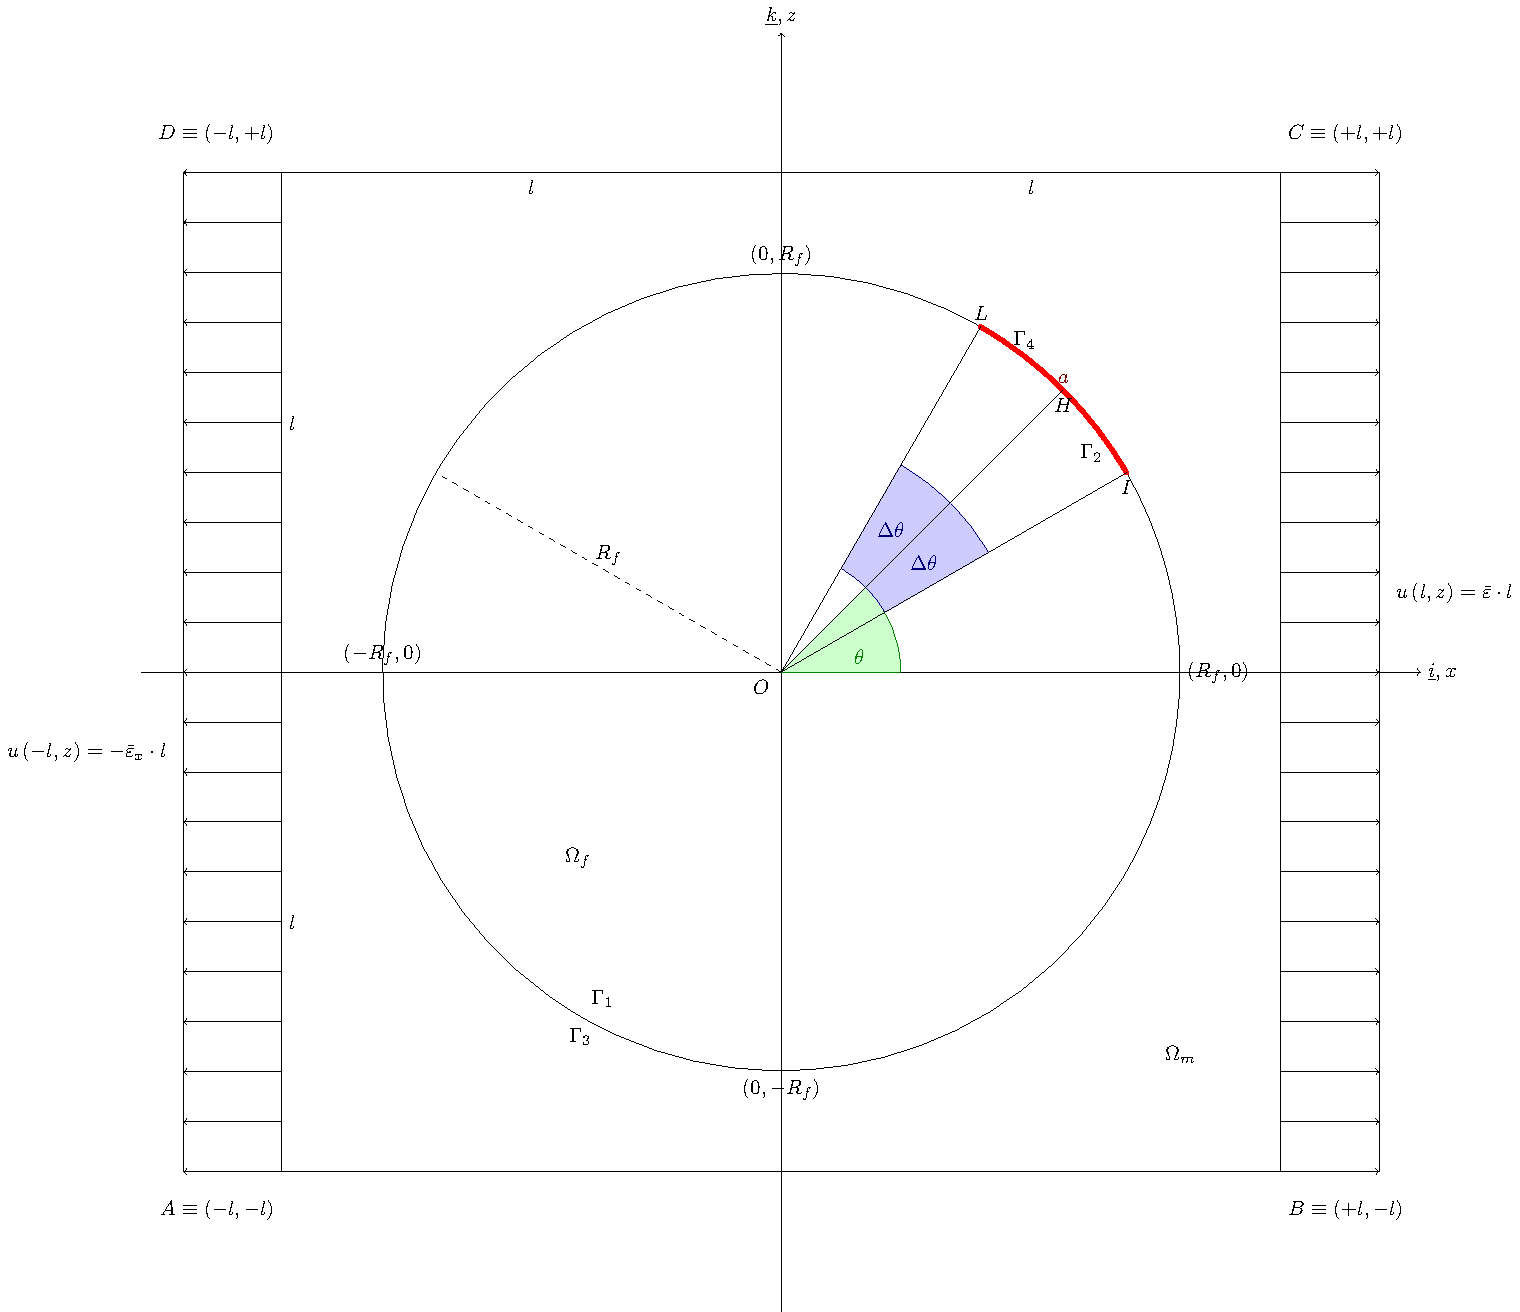
\includegraphics[height=0.7\textheight]{LEFM2DsRVEsFsDfreeBCULappAxialDispLR.pdf}
\caption{\scriptsize Simple RVE, BC: free.}
\label{fig:singleRVE-rigid}
\end{figure}
\end{frame}

\begin{frame}
\frametitle{\small Reference Models}
\vspace{-0.25cm}
\centering
\begin{figure}
\centering
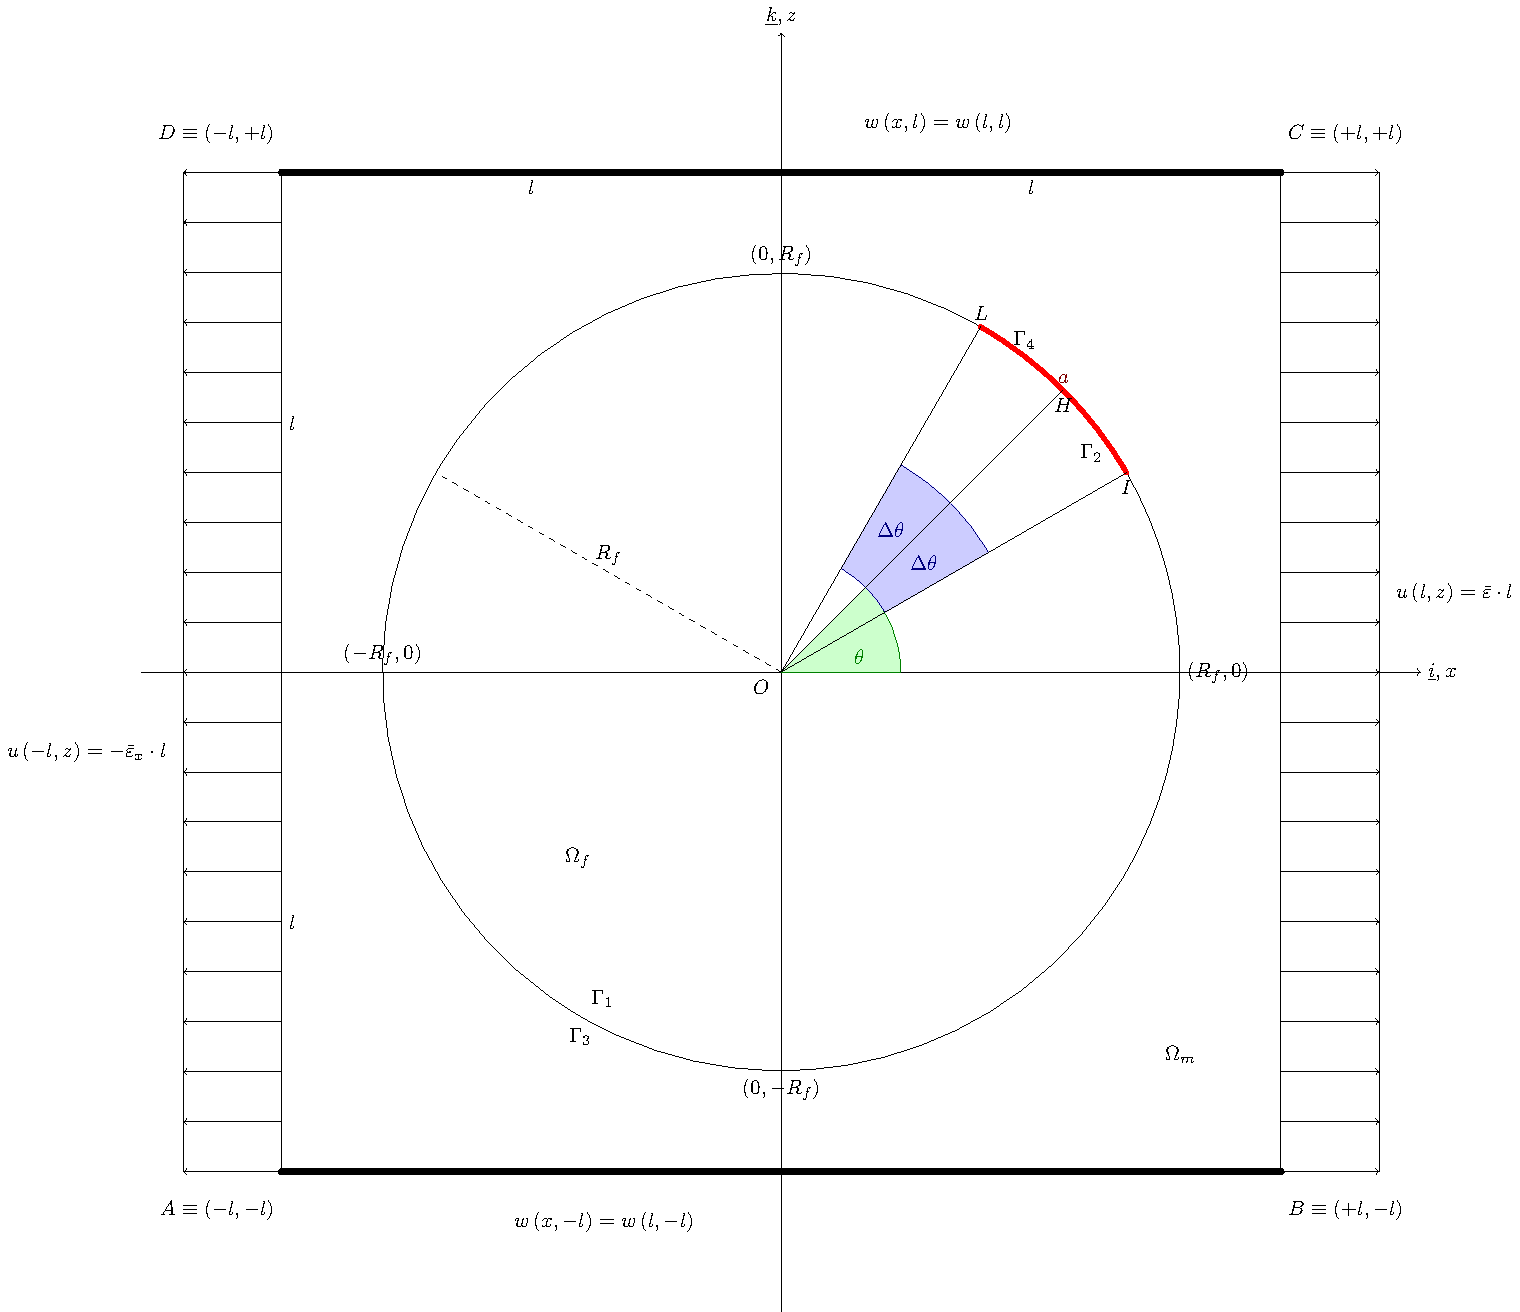
\includegraphics[height=0.7\textheight]{LEFM2DsRVEsFsDdepverdispBCULappAxialDispLR.pdf}
\caption{\scriptsize Simple RVE, BC: fixed vertical displacement.}
\label{fig:singleRVE-rigid}
\end{figure}
\end{frame}

\begin{frame}
\frametitle{\small Reference Models}
\vspace{-0.25cm}
\centering
\begin{figure}
\centering
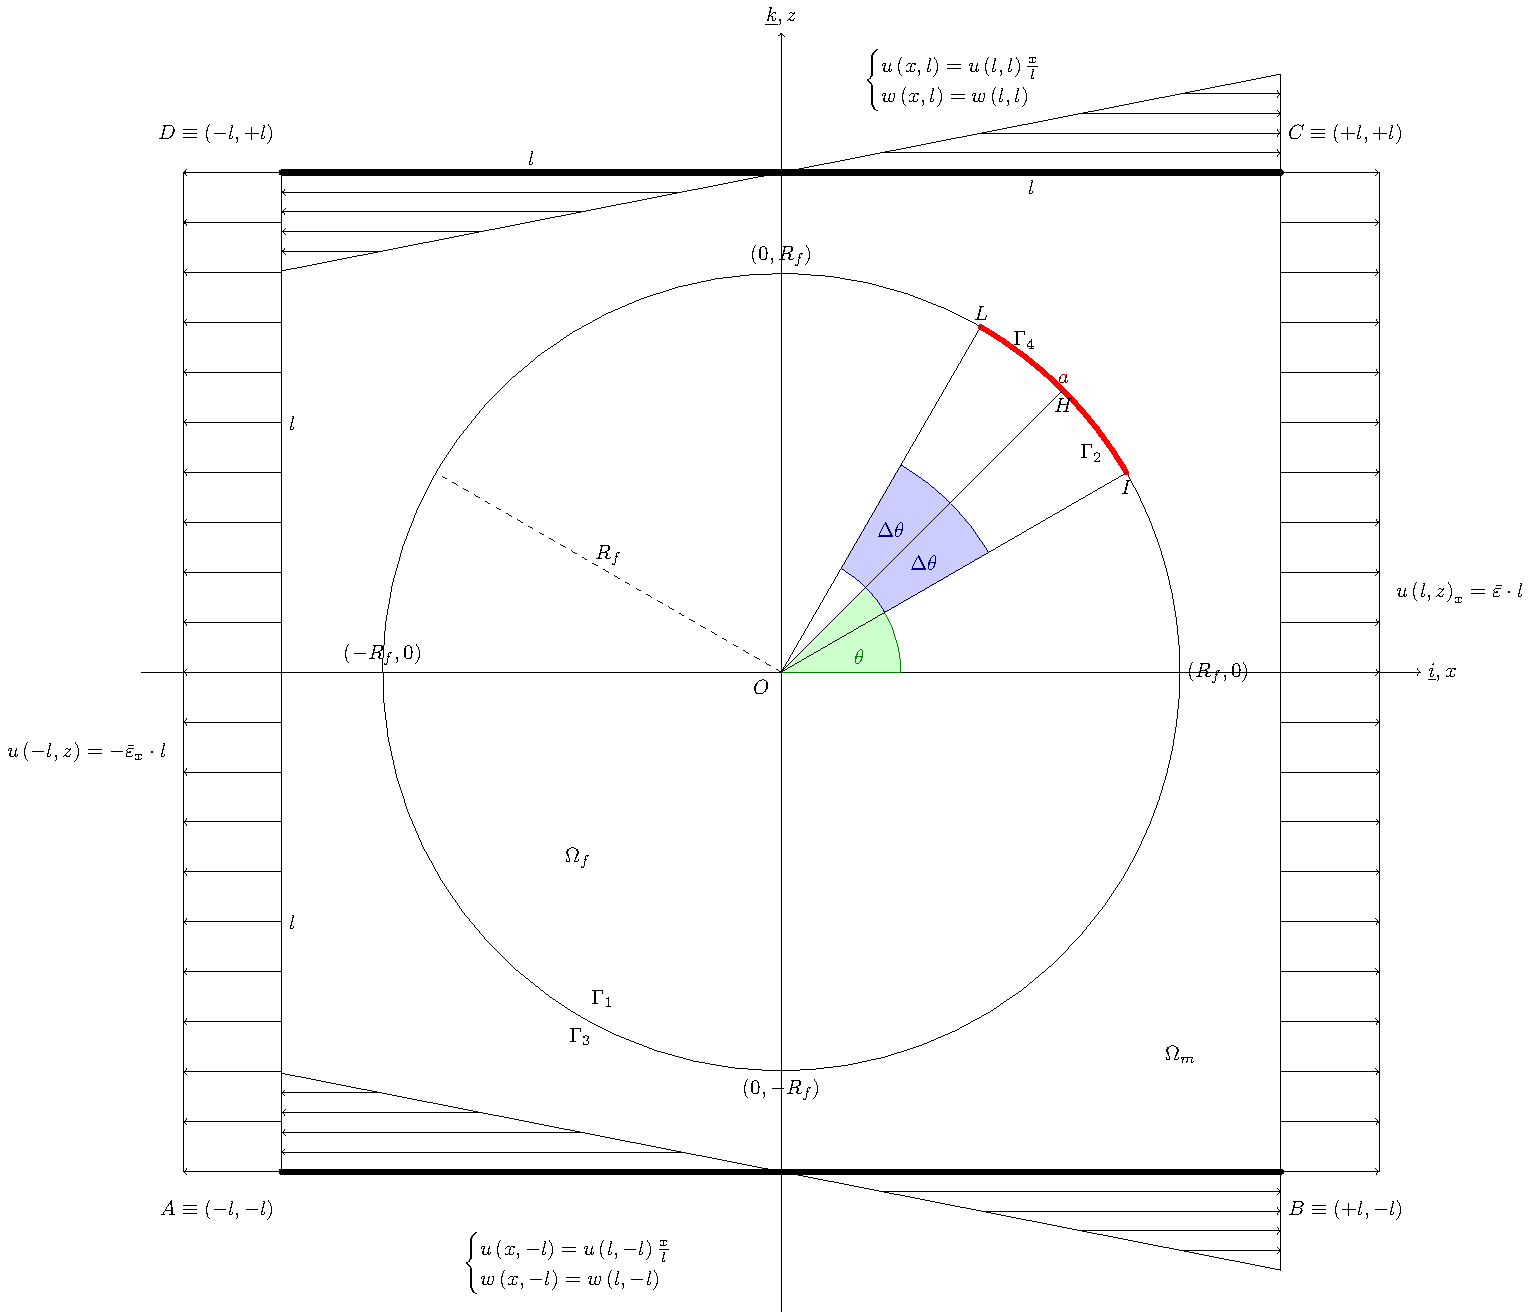
\includegraphics[height=0.7\textheight]{LEFM2DsRVEsFsDhomoBCULappAxialDispLR.pdf}
\caption{\scriptsize Simple RVE, BC: fixed vertical and homogeneous horizontal displacement.}
\label{fig:singleRVE-homo}
\end{figure}
\end{frame}

\subsection{Angular discretization}

\begin{frame}
\frametitle{\small Angular discretization}
\vspace{-0.7cm}
\centering
\captionsetup[figure]{font=scriptsize,labelfont=scriptsize}
\begin{figure}[!h]
\centering
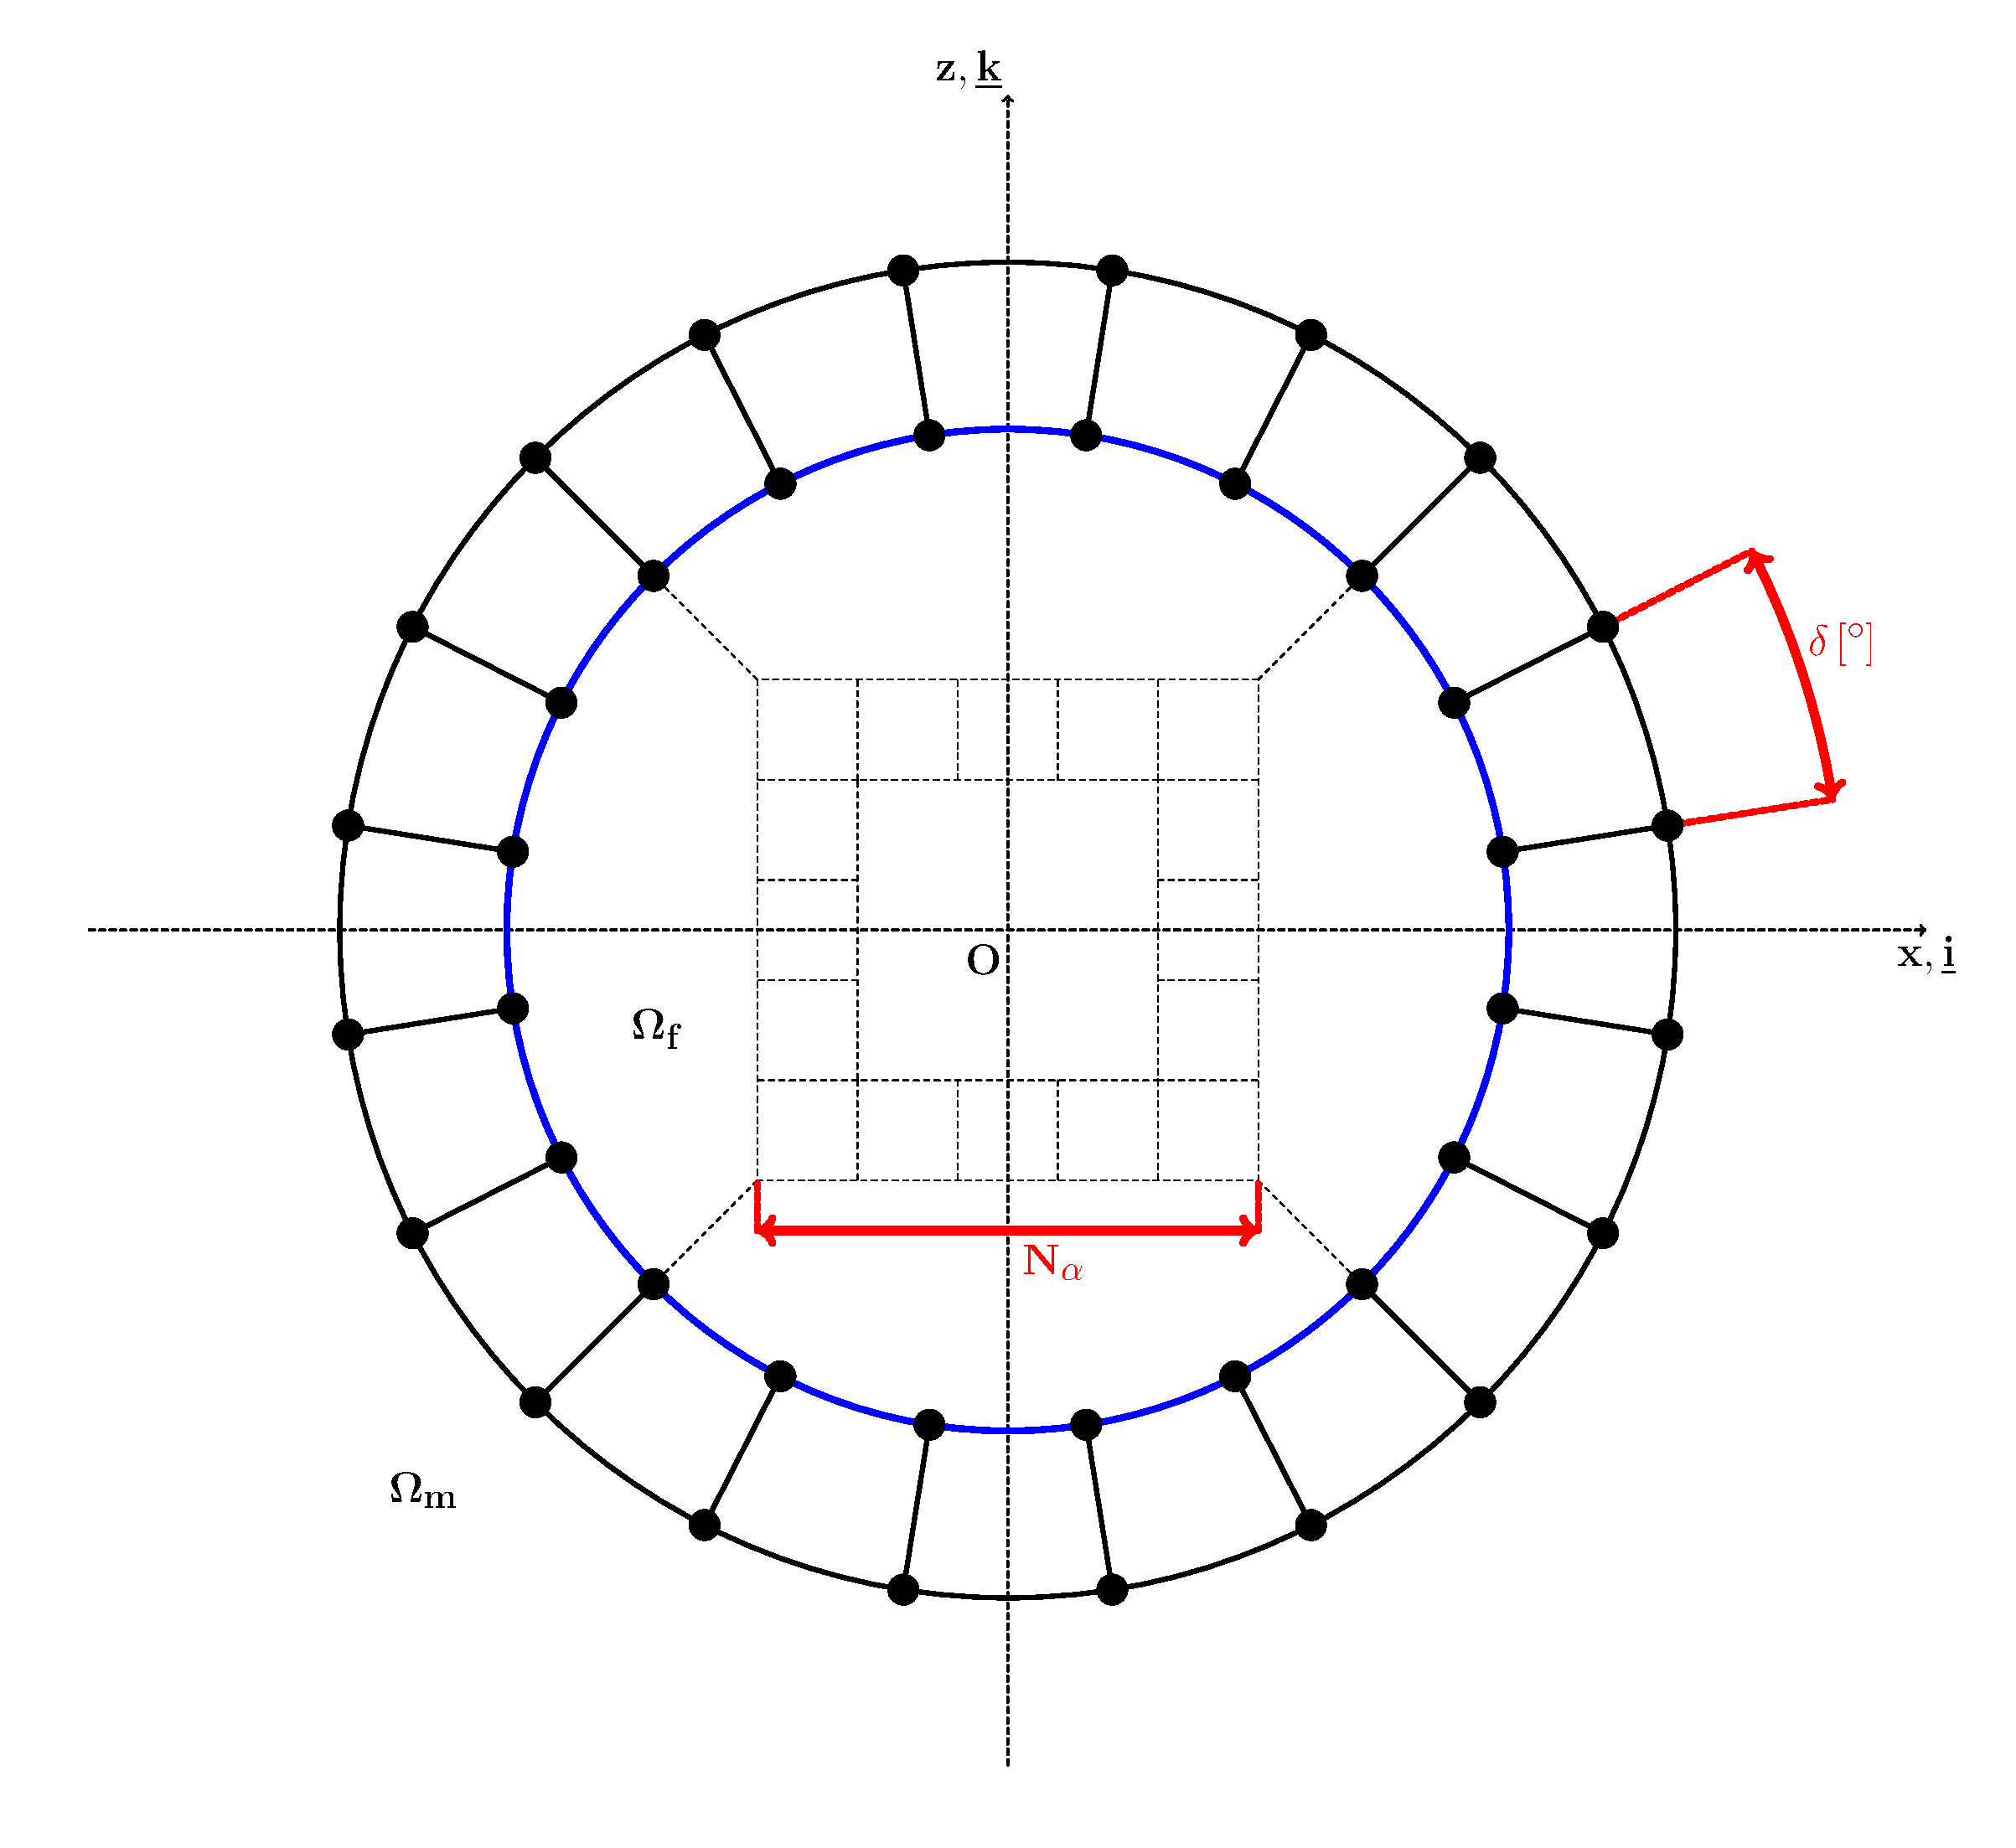
\includegraphics[height=0.7\textheight]{mesh-disc-at-interface.pdf}
  \caption{\scriptsize Angular discretization at fiber/matrix interface: $\delta=\frac{360^{\circ}}{4N_{\alpha}}$.}
  \label{fig:angu-discr-def}
\end{figure}
\end{frame}

\subsection{Material properties}

\begin{frame}
\frametitle{\small Material properties}
\vspace{-0.7cm}
\footnotesize
\centering
\captionsetup[figure]{font=scriptsize,labelfont=scriptsize}
\begin{table}[htbp]

  \centering
  %\caption{Single phase properties summary.}
    \begin{tabular}{cccc}

    \textbf{Material} & \textbf{$E\left[GPa\right]$}\ & \textbf{$G\left[GPa\right]$} & \textbf{$\nu\left[-\right]$} \\[3pt]
    \midrule\\[12pt]
    Glass fiber    & 70,0  & 29,2   & 0,2  \\[16pt]
    Epoxy    & 3,5    & 1,25   & 0,4  

    \end{tabular}%
  \label{tab:phaseprop}%
\end{table}%
\end{frame}

\subsection{Evaluation of $G_{0}$}
\begin{frame}
\frametitle{\small Evaluation of $G_{0}$}
\vspace{-0.7cm}
\footnotesize
\centering
\captionsetup[figure]{font=scriptsize,labelfont=scriptsize}
\begin{equation}
G_{0}=\pi R_{f}\sigma^{2}_{0}\frac{1+k_{m}}{8G_{m}}
\end{equation}
\begin{equation}
k_{m}=3-4\nu_{m}
\end{equation}
\begin{equation}
\sigma_{0}^{undamaged}=\frac{E_{m}}{1-\nu^{2}_{m}}\varepsilon_{xx}
\end{equation}%
\end{frame}

\subsection{VCCT}
\begin{frame}
\frametitle{\small VCCT  in Forces}
\vspace{-0.5cm}
\tiny
\centering
\captionsetup[figure]{font=scriptsize,labelfont=scriptsize}
\begin{equation}
\Delta u = \left(x^{fiber, def}_{\text{1 element before crack tip}}-x^{fiber, undef}_{\text{1 element before crack tip}}\right)-\left(x^{matrix, def}_{\text{1 element before crack tip}}-x^{matrix, undef}_{\text{1 element before crack tip}}\right)
\end{equation}

\begin{equation}
\Delta w = \left(z^{fiber, def}_{\text{1 element before crack tip}}-z^{fiber, undef}_{\text{1 element before crack tip}}\right)-\left(z^{matrix, def}_{\text{1 element before crack tip}}-z^{matrix, undef}_{\text{1 element before crack tip}}\right)
\end{equation}

\begin{equation}
\beta=\arctan{\left(\frac{z^{matrix, def}_{\text{crack tip}}}{x^{matrix, def}_{\text{crack tip}}}\right)}
\end{equation}

\begin{equation}
\Delta_{r}=\cos{\left(\beta\right)}\Delta u+\sin{\left(\beta\right)}\Delta w\qquad\Delta_{\theta}=-\sin{\left(\beta\right)}\Delta u+\cos{\left(\beta\right)}\Delta w
\end{equation}

\begin{equation}
F_{r}=\cos{\left(\beta\right)}F^{reaction}_{x}+\sin{\left(\beta\right)}F^{reaction}_{z}\qquad F_{\theta}=-\sin{\left(\beta\right)}F^{reaction}_{x}+\cos{\left(\beta\right)}F^{reaction}_{z}
\end{equation}

\begin{equation}
G_{I}=\frac{1}{2}\frac{F_{r}\Delta_{r}}{R_{f}\delta}\qquad G_{II}=\frac{1}{2}\frac{F_{\theta}\Delta_{\theta}}{R_{f}\delta}\qquad b=1.0\leftrightarrow\Delta A = bR_{f}\delta
\end{equation}
\end{frame}

\section[$\sigma_{xx}\left(x=L,z\right)$]{Normal stress distribution at the loaded boundary}

\begin{frame}
\frametitle{\small $\sigma_{xx}\left(x=L,z\right)$ for $Vf_{f}=0.001$, $\frac{L}{R_{f}}\sim28$ and $\delta=0.4^{\circ}$}
\vspace{-0.5cm}
\centering
\captionsetup[figure]{font=scriptsize,labelfont=scriptsize}
\begin{figure}[!h]
\centering
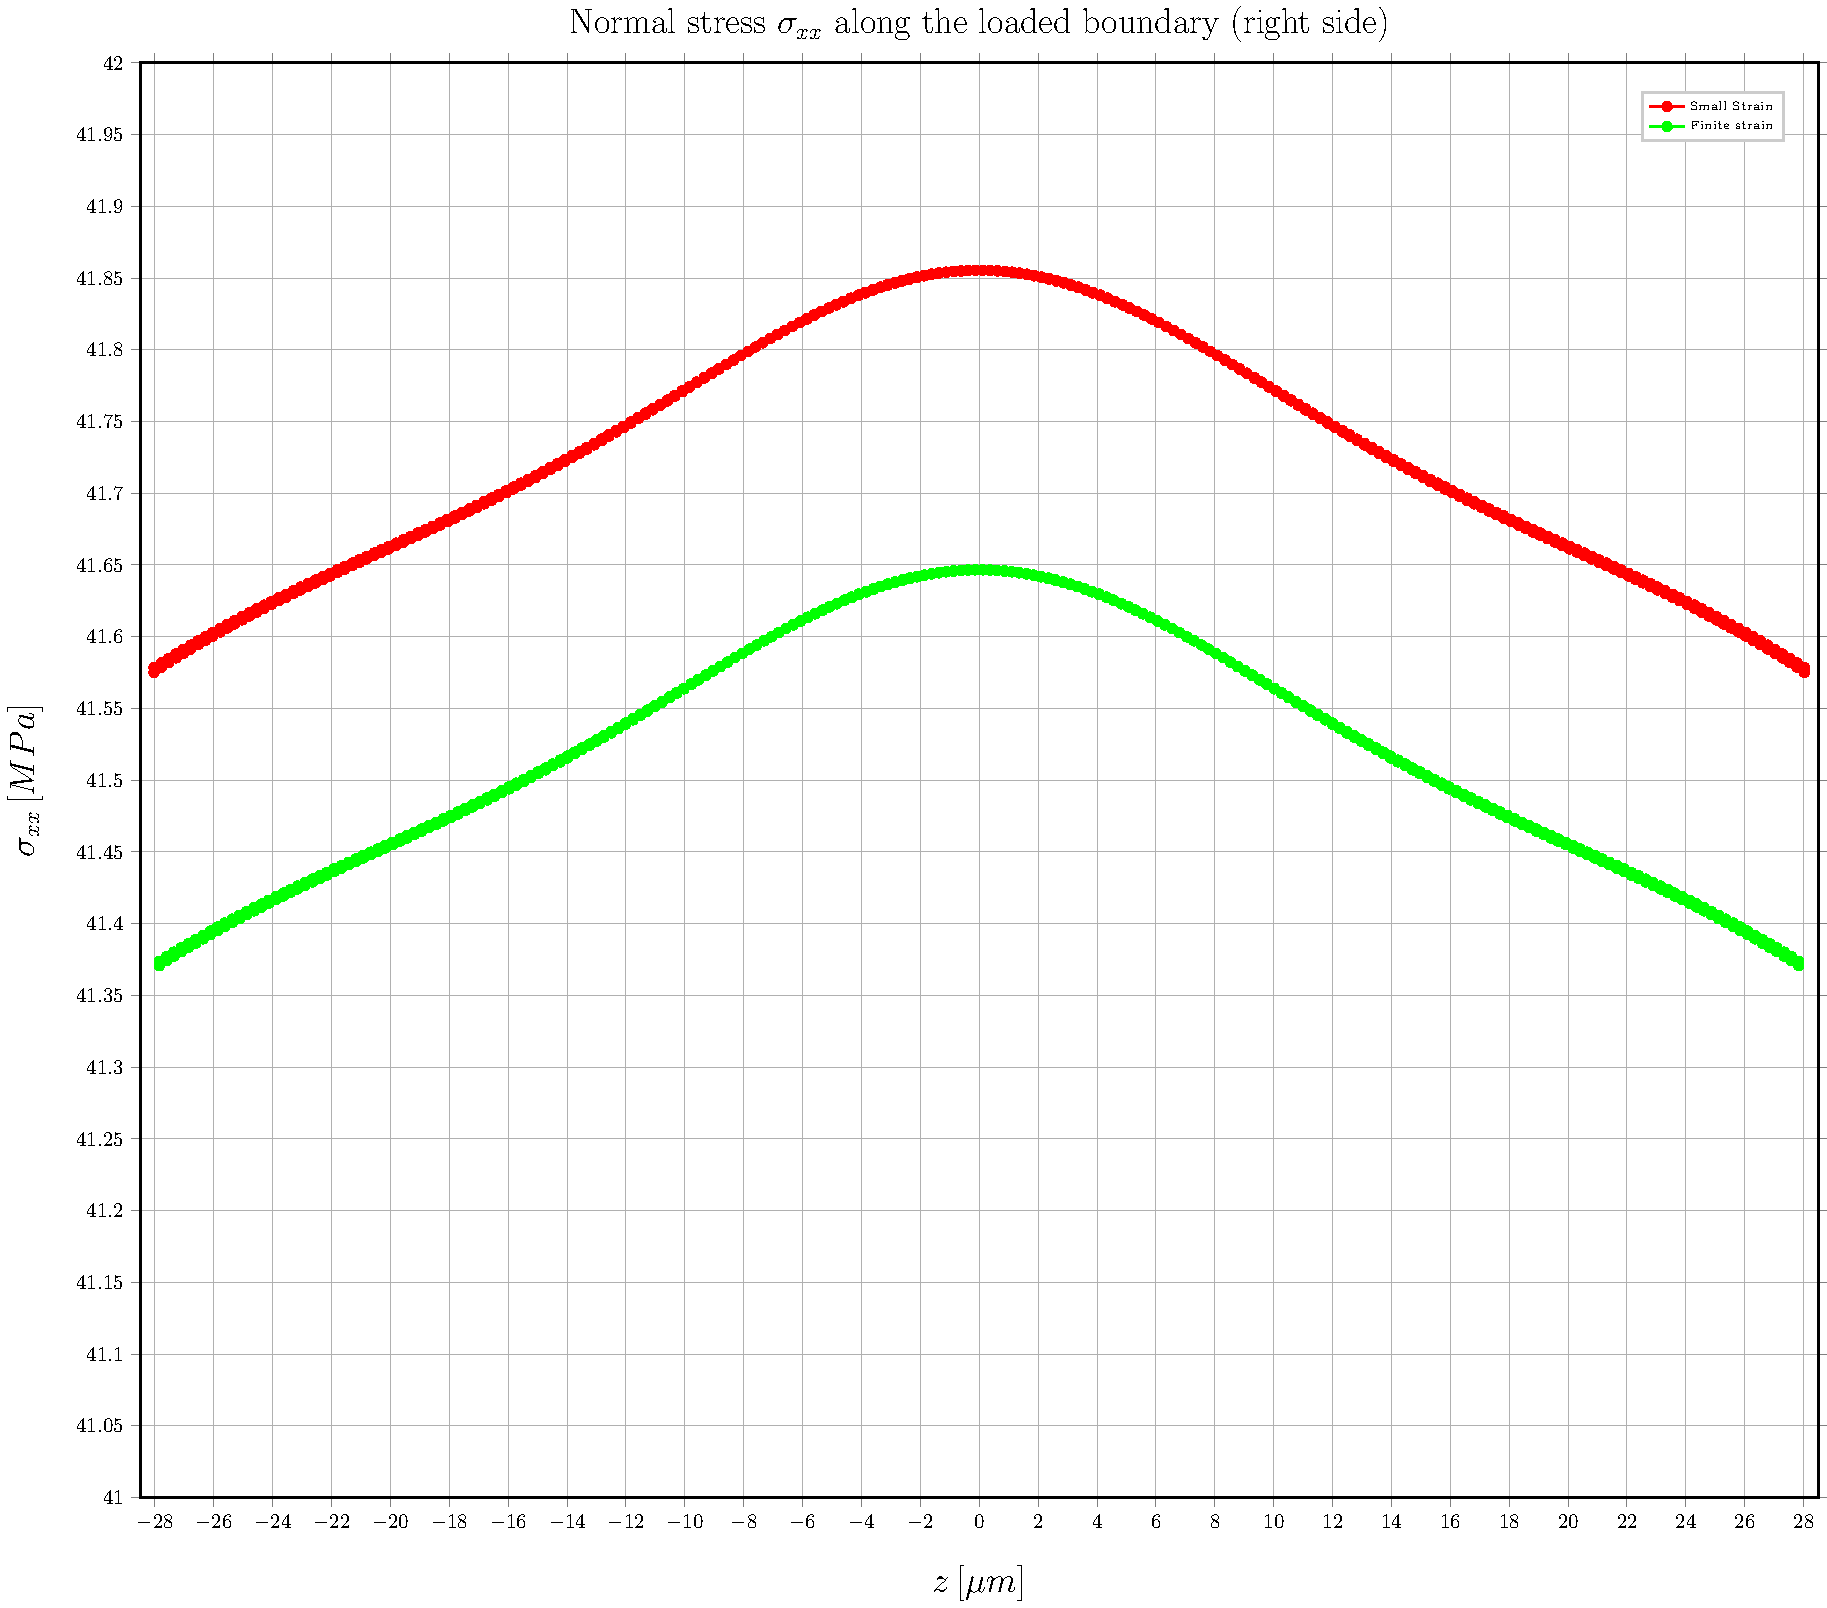
\includegraphics[height=0.7\textheight]{2017-06-23_AbqRunSummary_SingleFiberEqRfFiniteStrain_sigmaatboundary_Summary.pdf}
  \caption{\scriptsize In red small strain FEM, in green finite strain FEM.}
  \label{fig:res1}
\end{figure}
\end{frame}

\begin{frame}
\frametitle{\small $\sigma_{xx}\left(x=L,z\right)$ for $Vf_{f}=0.000079$, $\frac{L}{R_{f}}\sim100$ and $\delta=0.4^{\circ}$}
\vspace{-0.5cm}
\centering
\captionsetup[figure]{font=scriptsize,labelfont=scriptsize}
\begin{figure}[!h]
\centering
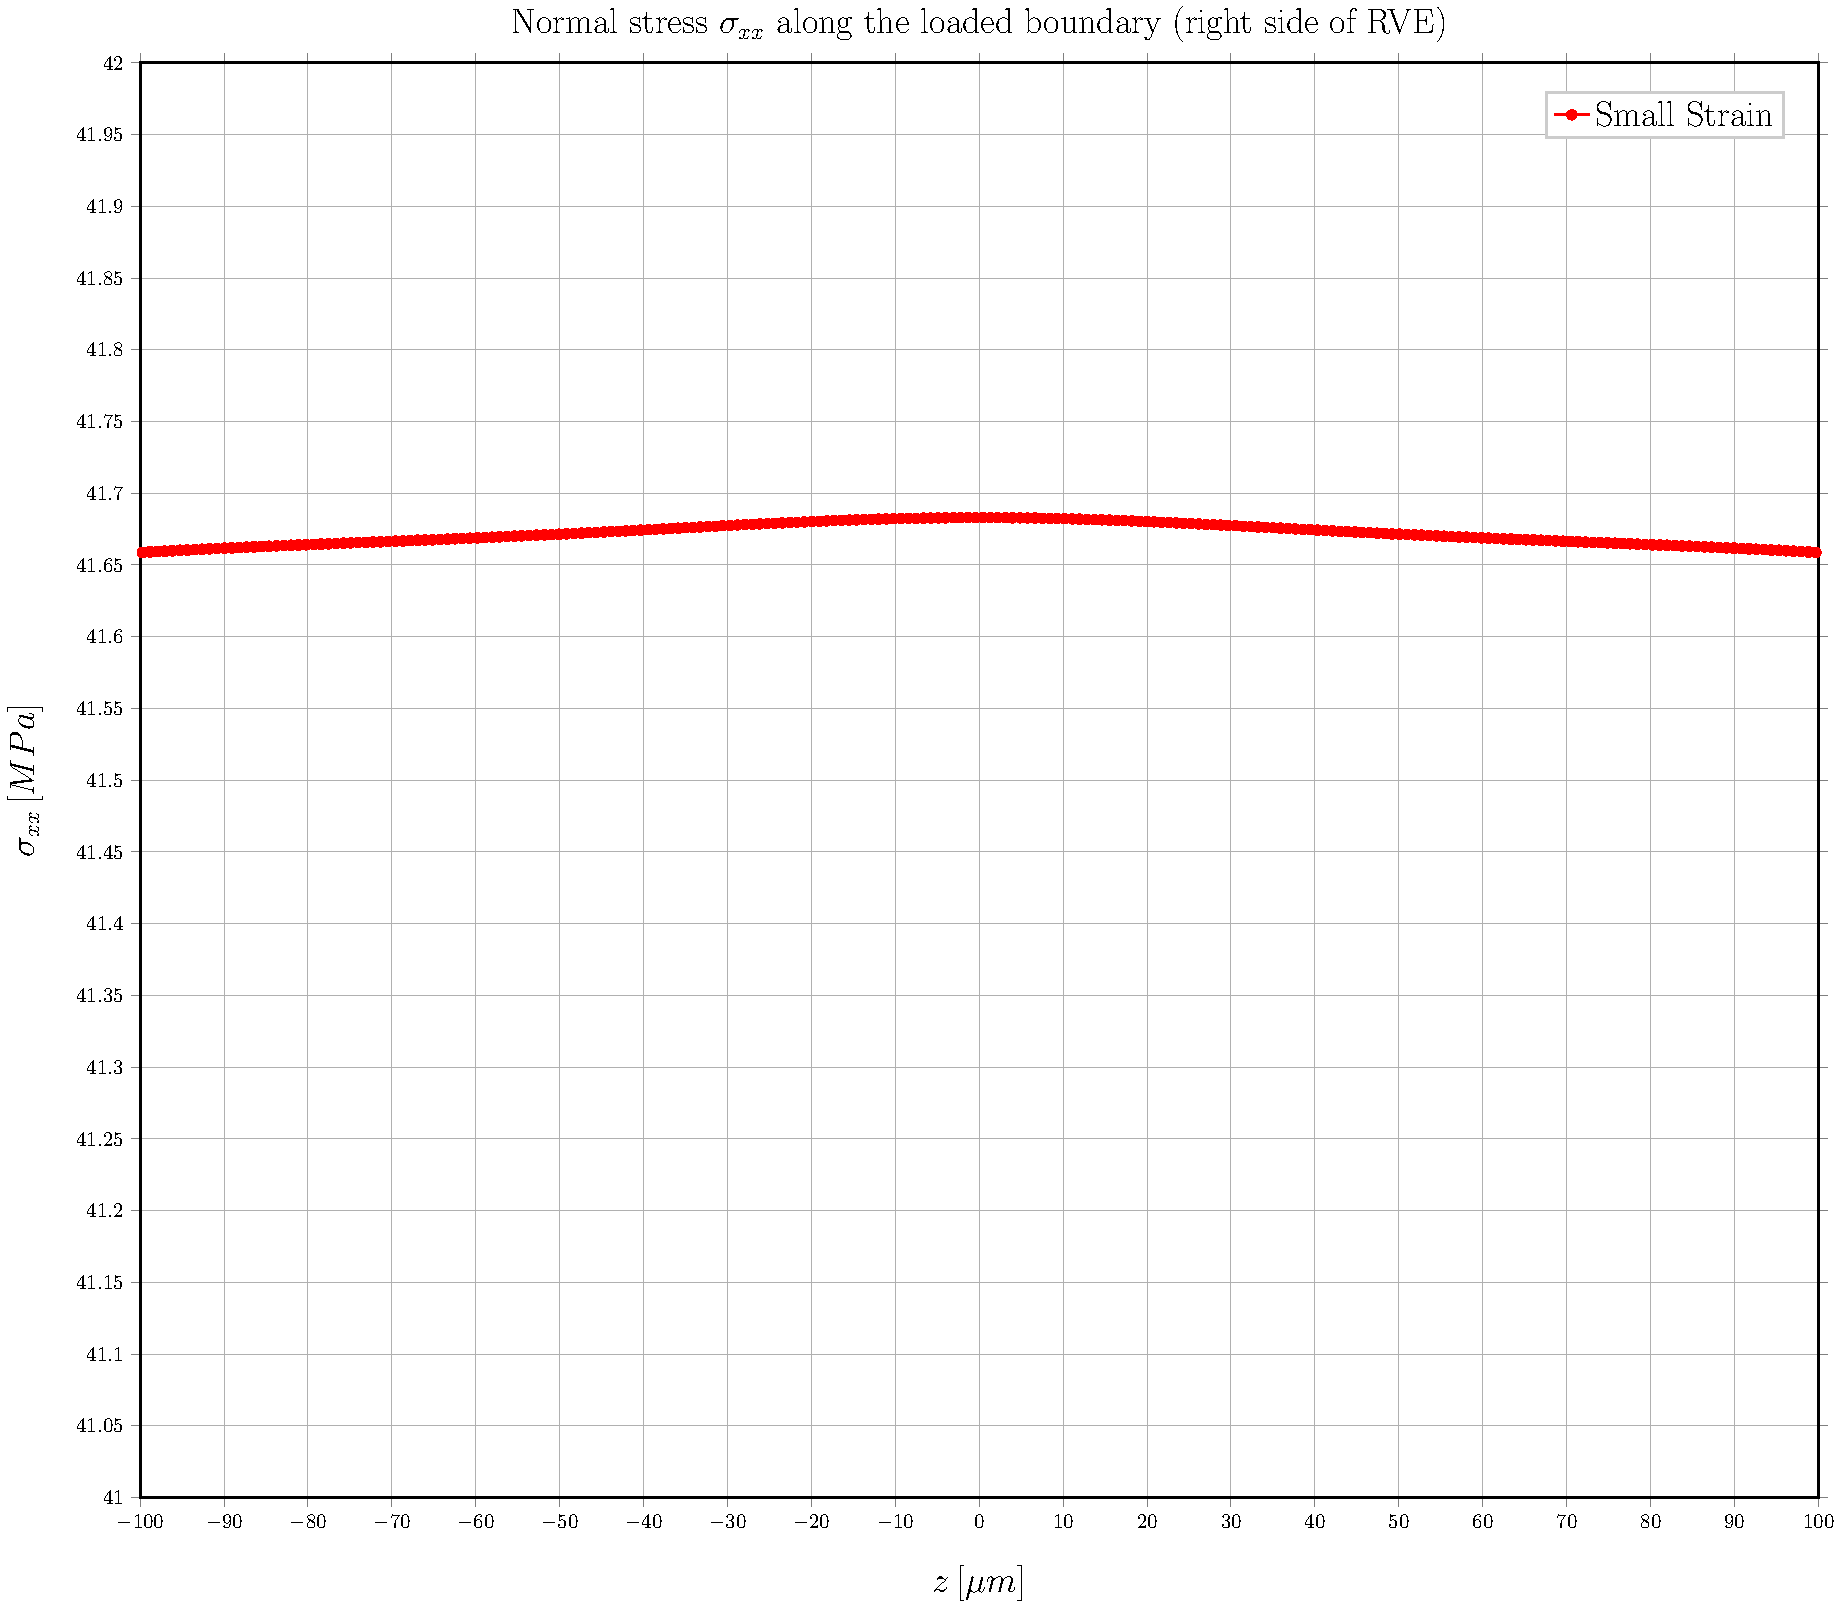
\includegraphics[height=0.7\textheight]{2017-06-16_AbqRunSummary_SingleFiberEqRfSmallStrain-D0-4_sigmaatboundary_Summary.pdf}
  \caption{\scriptsize In red small strain FEM.}
  \label{fig:res1}
\end{figure}
\end{frame}

\begin{frame}
\frametitle{\small Conclusions}
\vspace{-0.5cm}
\centering
\begin{itemize}[label=\ding{212}]
\item Maximum and minimum are equal due to symmetry
\item For $\frac{L}{R_{f}}\sim 28$ in small strain, the relative difference between maximum/minimum and mean value is $0.34\%$
\item For $\frac{L}{R_{f}}\sim 28$ in finite strain, the relative difference between maximum/minimum and mean value is $0.33\%$ 
\item For $\frac{L}{R_{f}}\sim 100$ in small strain, the relative difference between maximum/minimum and mean value is $0.03\%$ 
\item The stress at the boundary can thus be effectively approximated as constant and equal to the mean value
\end{itemize}
\end{frame}

\section{$\sigma_{0}$ and $G_{0}$}

\begin{frame}
\frametitle{\small $\sigma_{0}$ for $Vf_{f}=0.001$, $\frac{L}{R_{f}}\sim28$ and $\delta=0.4^{\circ}$}
\vspace{-0.5cm}
\centering
\captionsetup[figure]{font=scriptsize,labelfont=scriptsize}
\begin{figure}[!h]
\centering
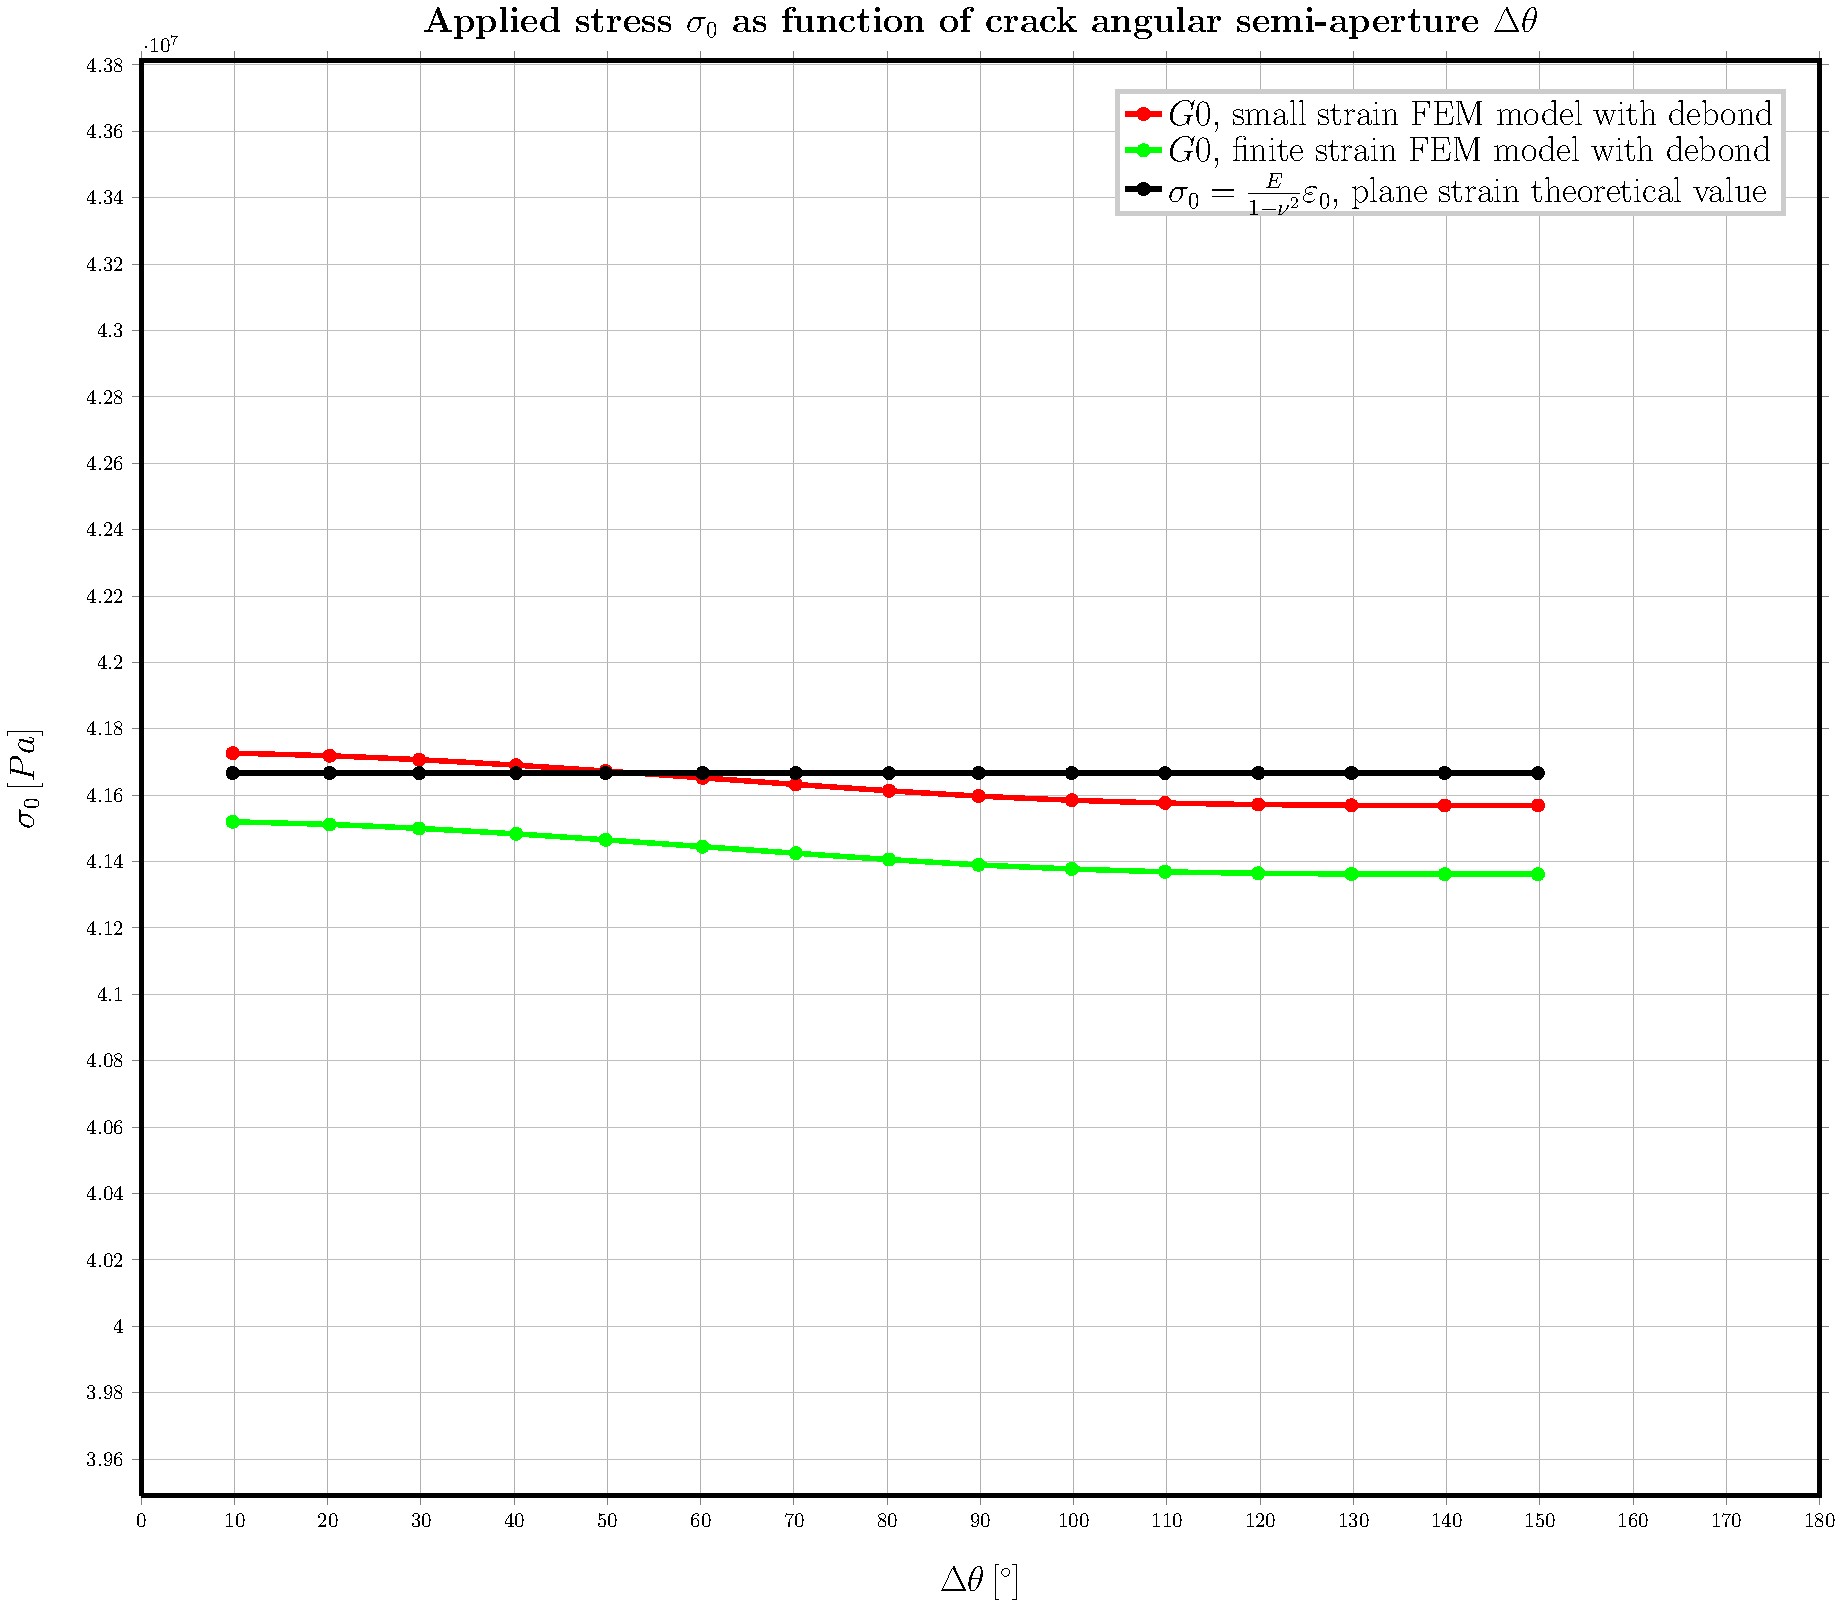
\includegraphics[height=0.7\textheight]{2017-06-23_AbqRunSummary_SingleFiberEqRfSmallFiniteStrain_sigma-inf_Summary.pdf}
  \caption{\scriptsize In red small strain FEM, in green finite strain FEM, in black $\sigma_{0}=\frac{E}{1-\nu^{2}}\varepsilon$.}
  \label{fig:res1}
\end{figure}
\end{frame}

\begin{frame}
\frametitle{\small $G_{0}$ for $Vf_{f}=0.001$, $\frac{L}{R_{f}}\sim28$ and $\delta=0.4^{\circ}$}
\vspace{-0.5cm}
\centering
\captionsetup[figure]{font=scriptsize,labelfont=scriptsize}
\begin{figure}[!h]
\centering
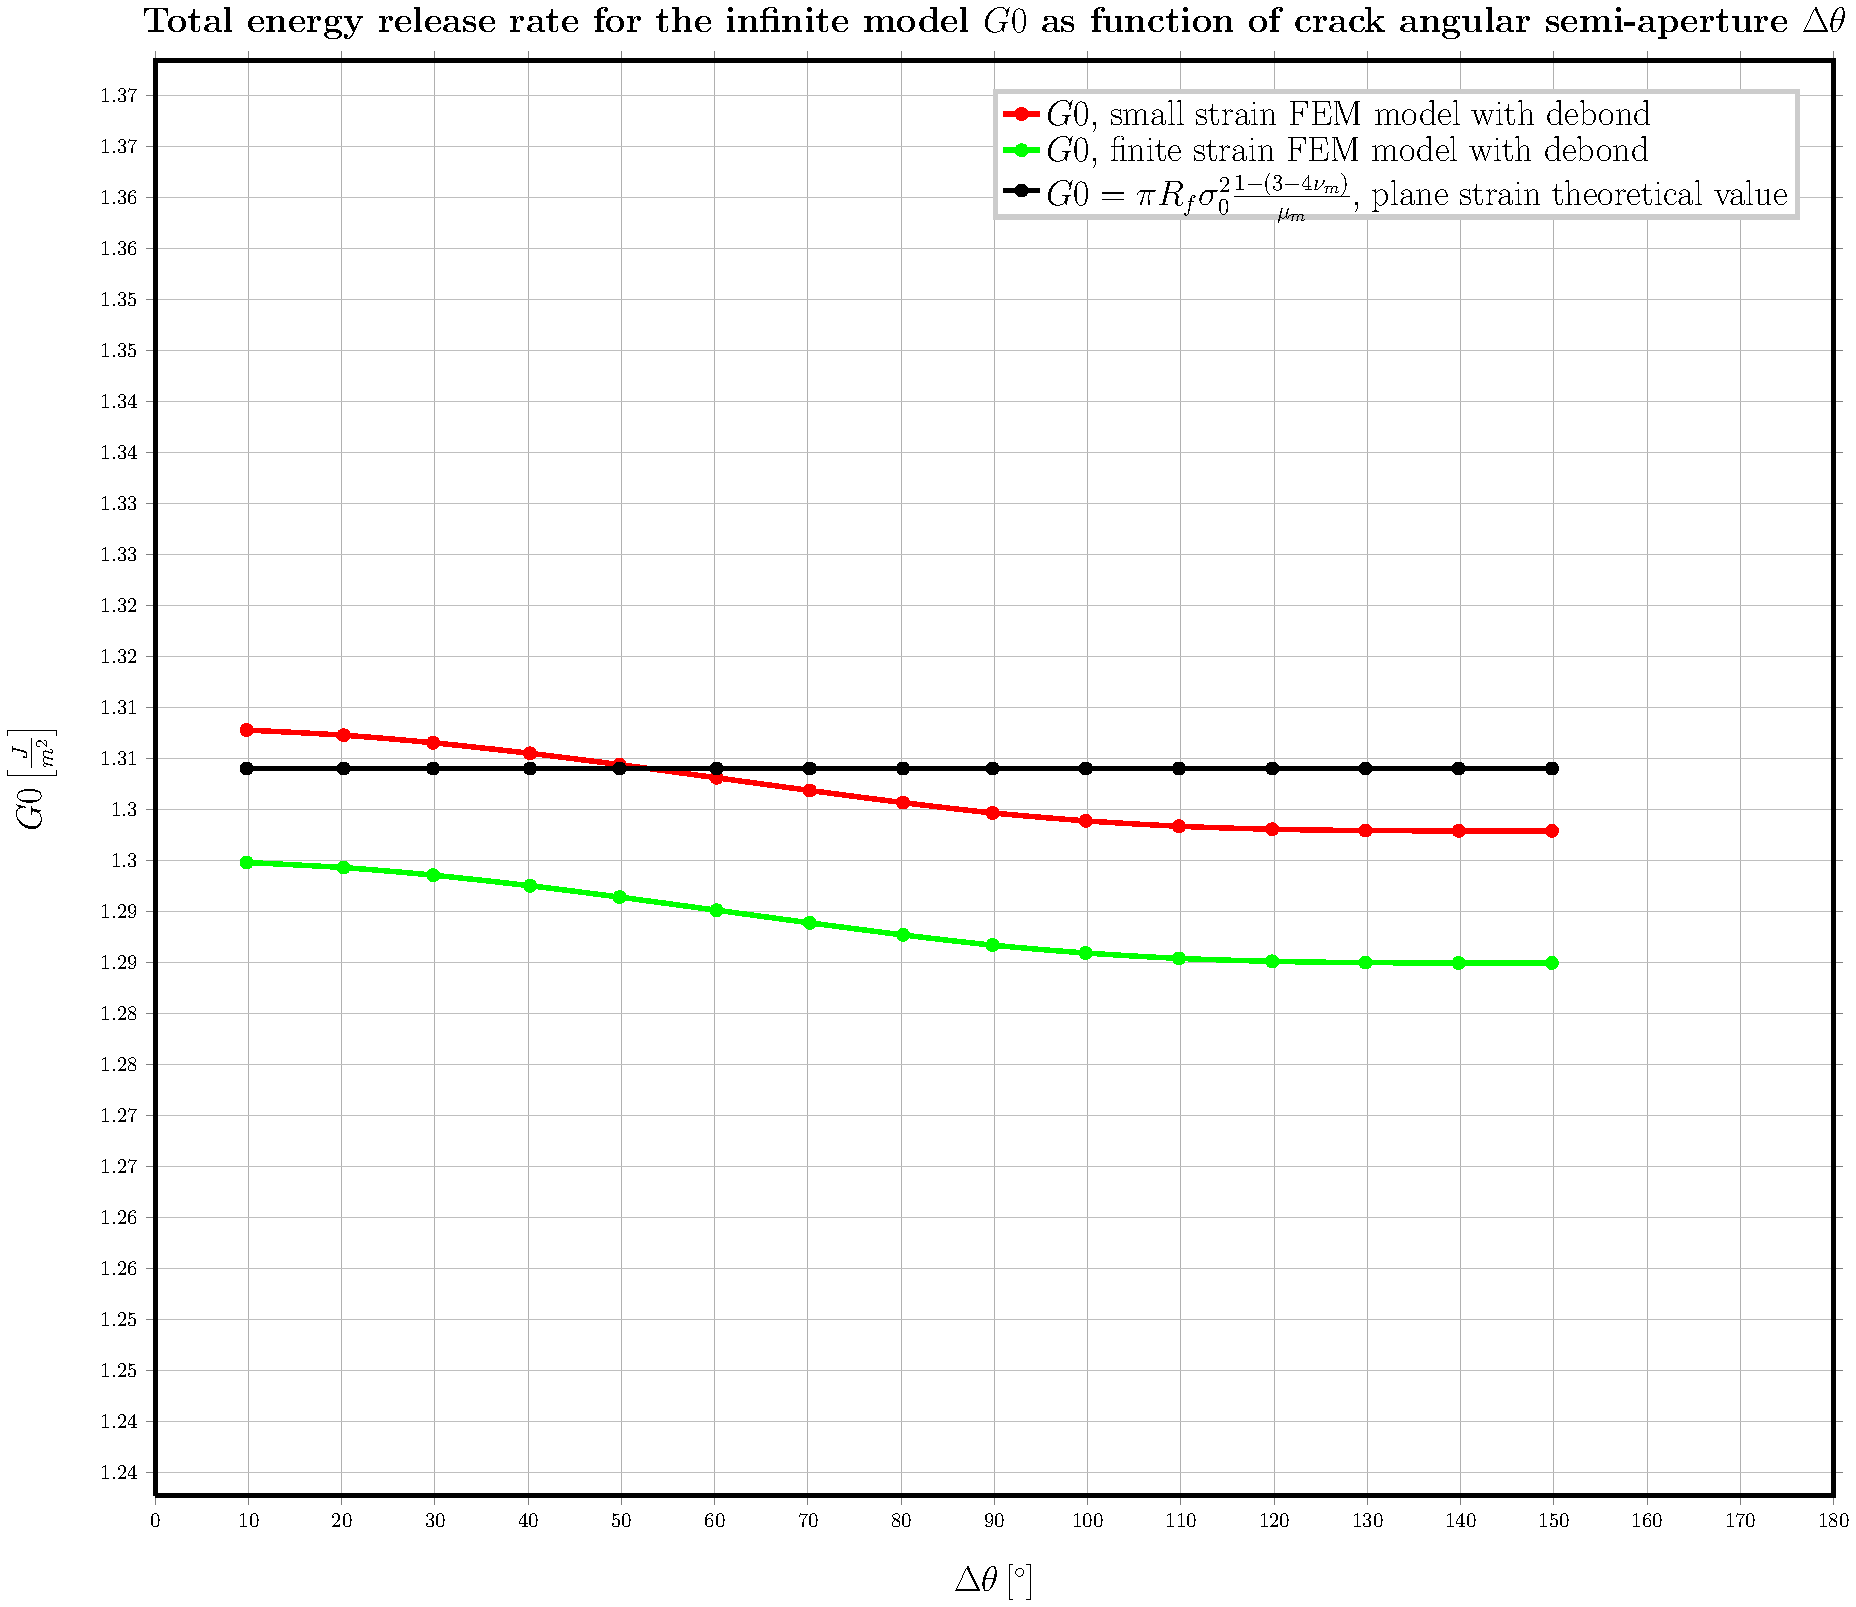
\includegraphics[height=0.7\textheight]{2017-06-23_AbqRunSummary_SingleFiberEqRfSmallFiniteStrain_G0_Summary.pdf}
  \caption{\scriptsize In red small strain FEM, in green finite strain FEM, in black $G_{0}$ calculated assuming $\sigma_{0}=\frac{E}{1-\nu^{2}}\varepsilon$.}
  \label{fig:res1}
\end{figure}
\end{frame}

\begin{frame}
\frametitle{\small $\sigma_{0}$ for $Vf_{f}=0.000079$, $\frac{L}{R_{f}}\sim100$ and $\delta=0.4^{\circ}$}
\vspace{-0.5cm}
\centering
\captionsetup[figure]{font=scriptsize,labelfont=scriptsize}
\begin{figure}[!h]
\centering
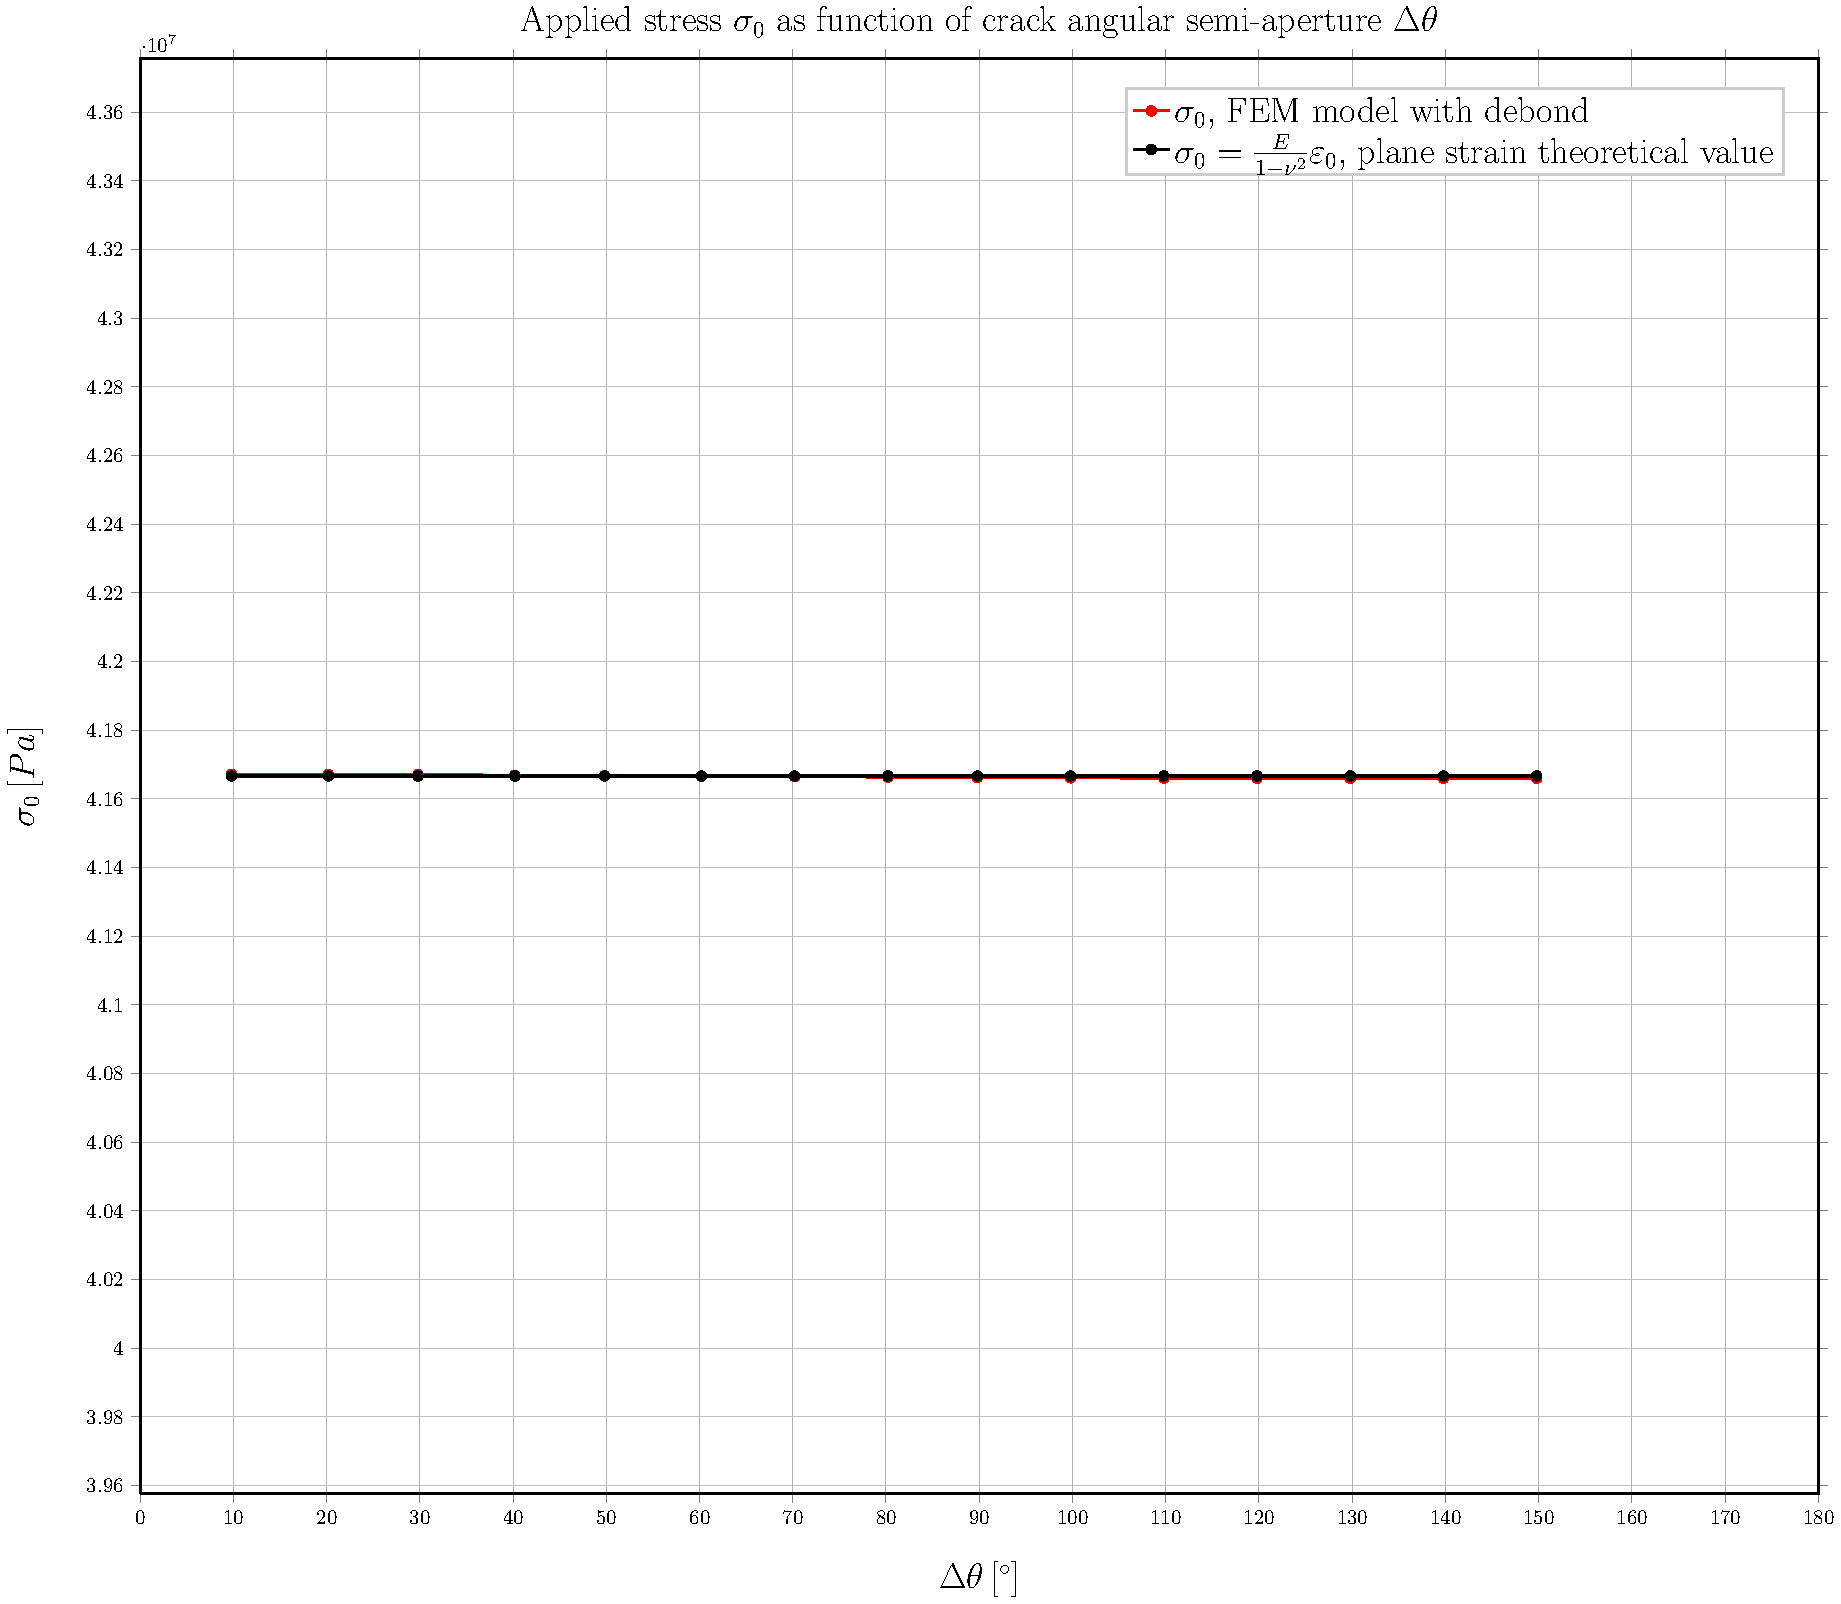
\includegraphics[height=0.7\textheight]{2017-06-16_AbqRunSummary_SingleFiberEqRfSmallStrain-D0-4_sigma-inf_Summary.pdf}
  \caption{\scriptsize In red small strain FEM, in black $\sigma_{0}=\frac{E}{1-\nu^{2}}\varepsilon$.}
  \label{fig:res1}
\end{figure}
\end{frame}

\begin{frame}
\frametitle{\small $G_{0}$ for $Vf_{f}=0.000079$, $\frac{L}{R_{f}}\sim100$ and $\delta=0.4^{\circ}$}
\vspace{-0.5cm}
\centering
\captionsetup[figure]{font=scriptsize,labelfont=scriptsize}
\begin{figure}[!h]
\centering
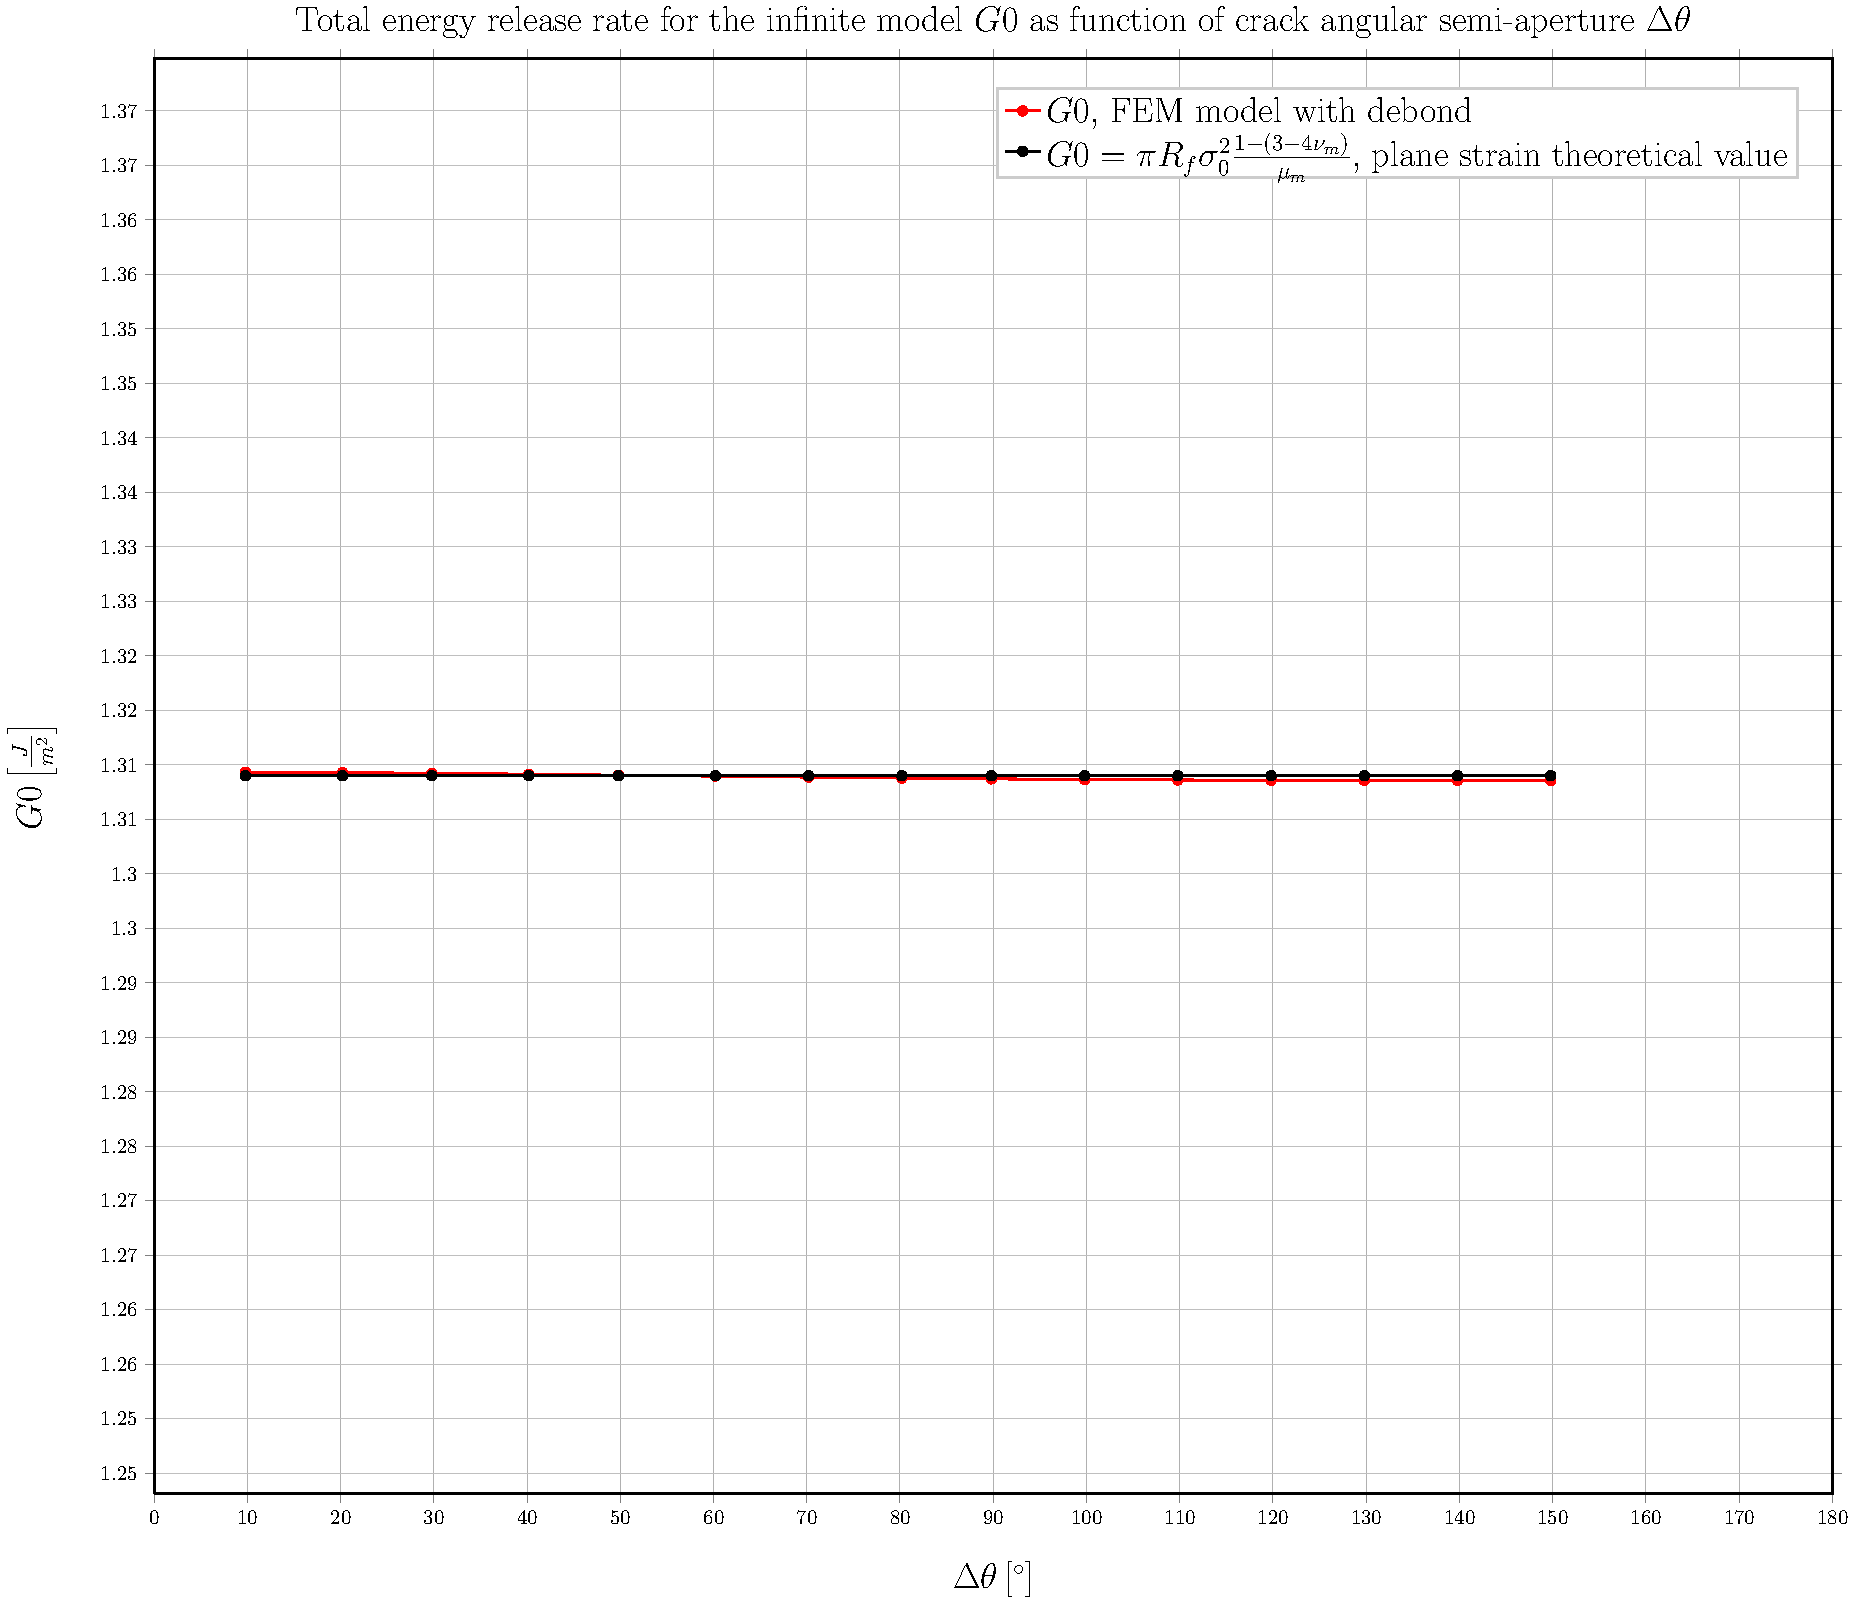
\includegraphics[height=0.7\textheight]{2017-06-16_AbqRunSummary_SingleFiberEqRfSmallStrain-D0-4_G0_Summary.pdf}
  \caption{\scriptsize In red small strain FEM, in black $G_{0}$ calculated assuming $\sigma_{0}=\frac{E}{1-\nu^{2}}\varepsilon$.}
  \label{fig:res1}
\end{figure}
\end{frame}

\begin{frame}
\frametitle{\small Conclusions}
\vspace{-0.5cm}
\centering
\begin{itemize}[label=\ding{212}]
\item $\sigma_{0}$ and $G_{0}$ depend on $\Delta\theta$ for finite sizes of the RVE
\item As the RVE size $\rightarrow\infty$, i.e. $\frac{L}{R_{f}}\rightarrow \infty$ ($\sim 100$), $\sigma_{0}$ and $G_{0}$ tend to the theoretical undamaged value given by $\sigma_{0}=\frac{E_{m}}{1-\nu_{m}^{2}}\varepsilon_{0}$
\item $\sigma_{0}$ and $G_{0}$ might be taken as a good measure of "infinetess" for strain-/displacement-controlled simulations
\item By selecting $\Delta\theta=10^{\circ}$ and running a parametric study with a comparatevely coarse mesh the minimum ratio  $\frac{L}{R_{f}}$ or equivalently maximum $Vf_{f}$ volume to have an infinite RVE could be found
\end{itemize}
\end{frame}

\section[FS \& SS]{Finite strain and small strain formulations}

\begin{frame}
\frametitle{\small $\frac{G_{\left(\cdot\cdot\right)}}{G_{0}}$ for $V_{f}=0.001$, $\frac{L}{R_{f}}\sim28$ and $\delta=0.4^{\circ}$}
\vspace{-0.5cm}
\centering
\captionsetup[figure]{font=scriptsize,labelfont=scriptsize}
\begin{figure}[!h]
\centering
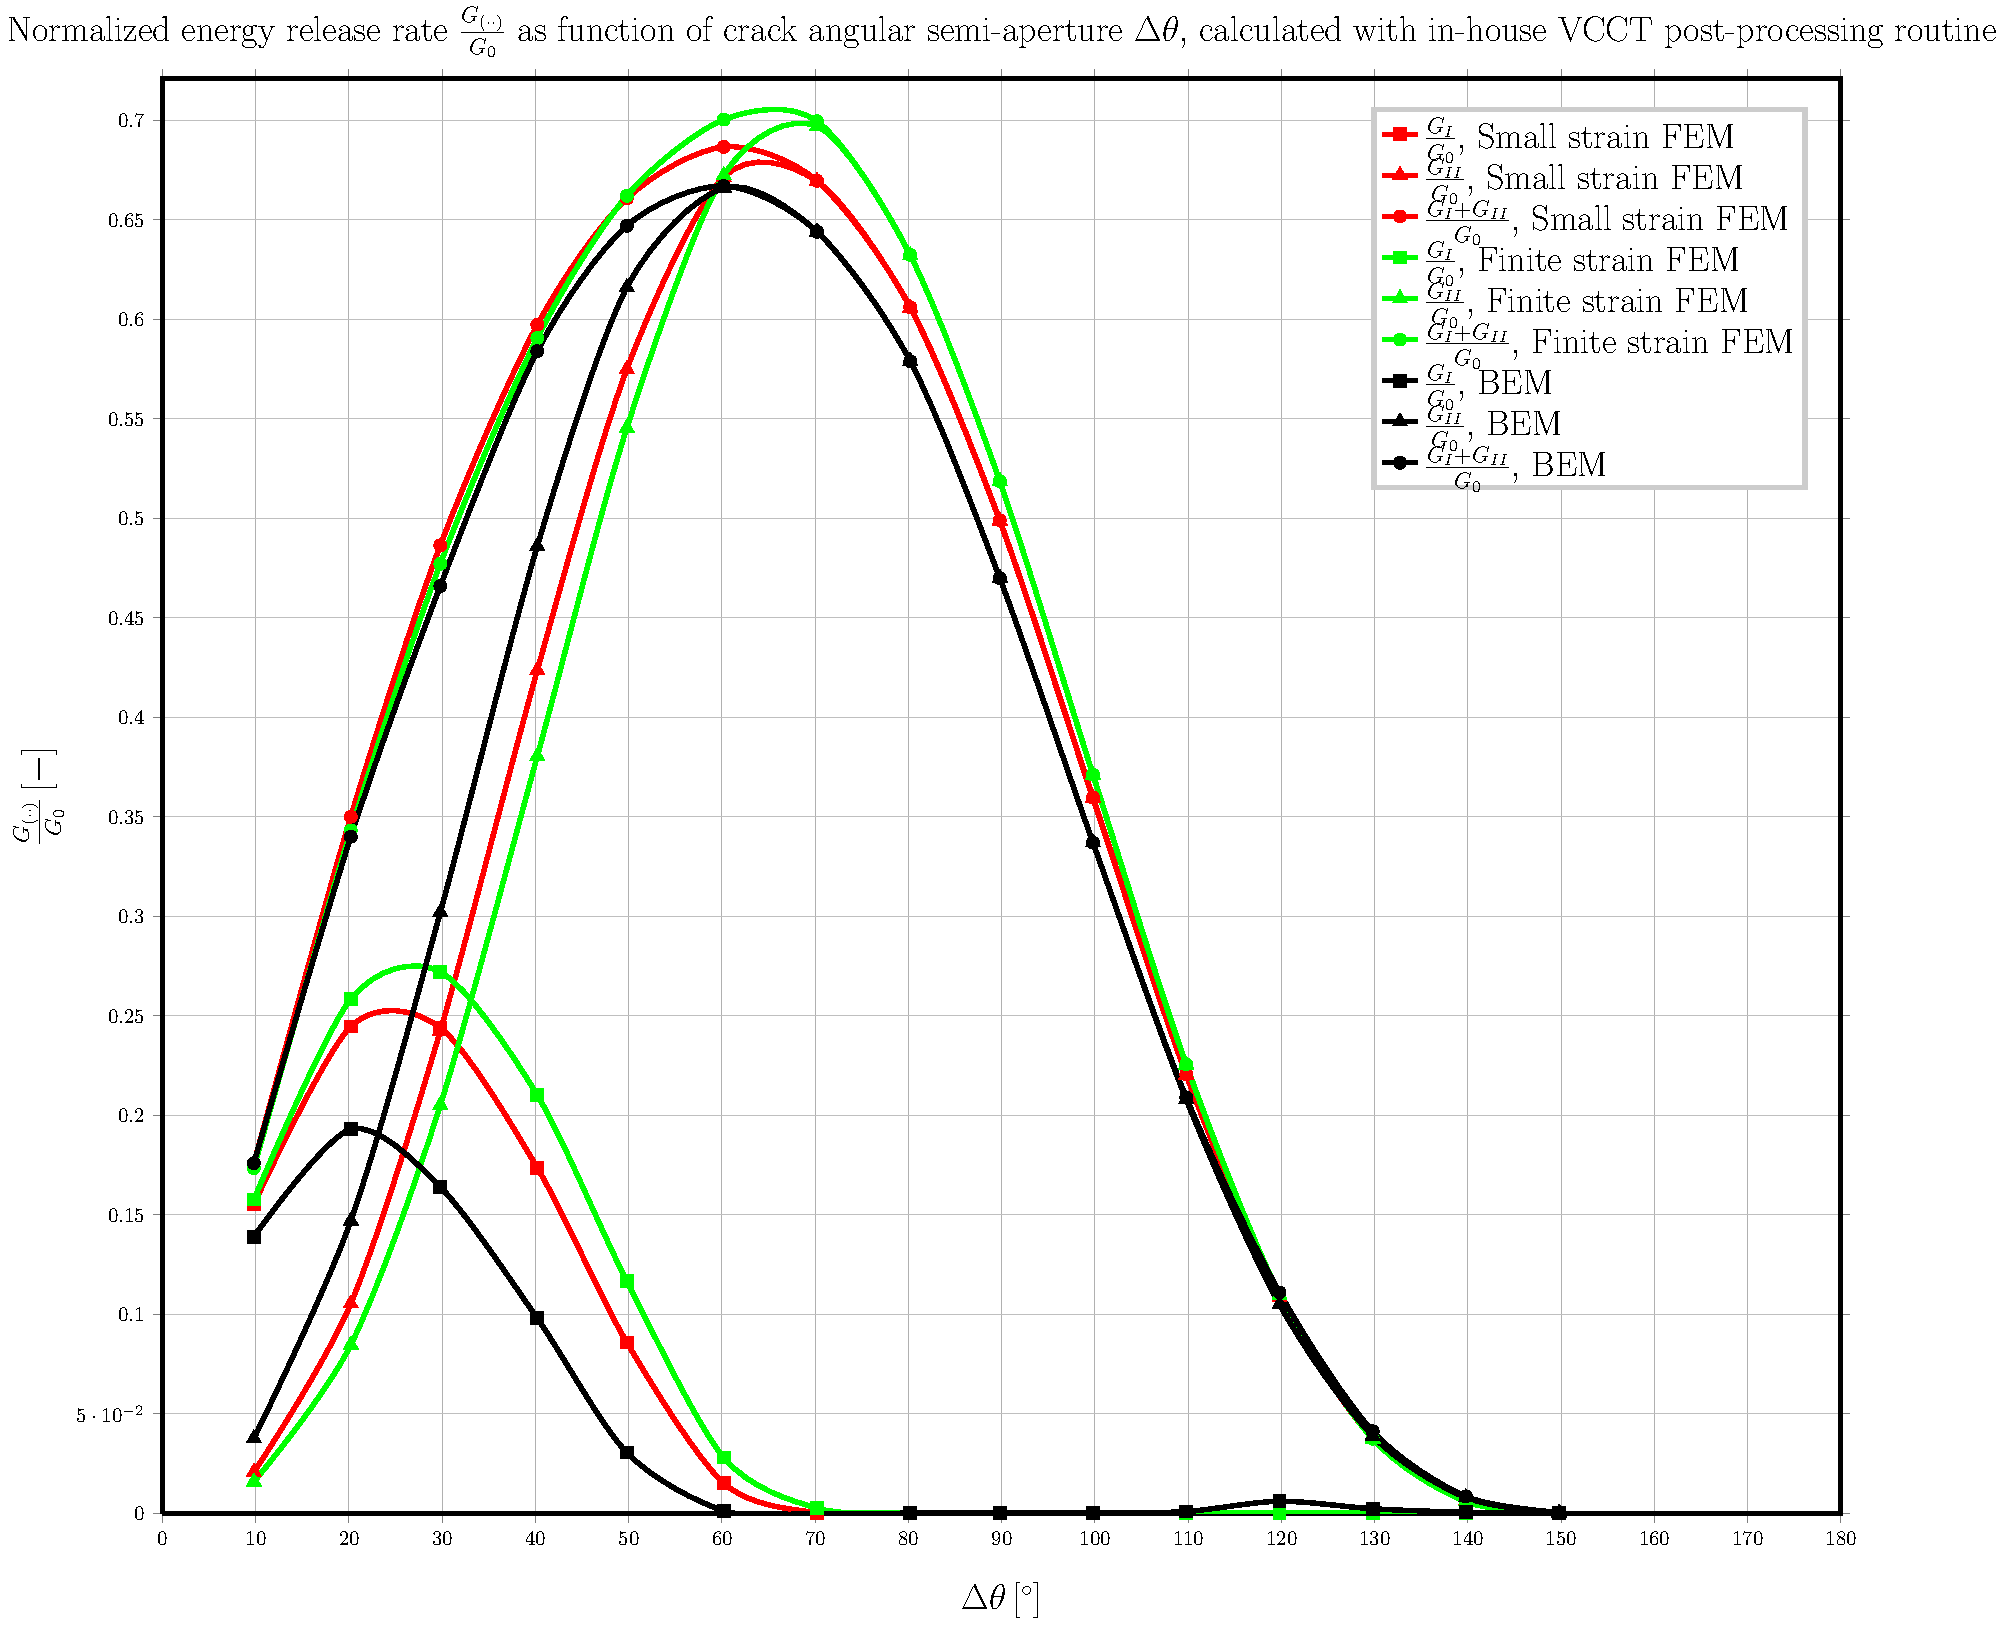
\includegraphics[height=0.7\textheight]{2017-06-23_AbqRunSummary_SingleFiberEqRfSmallFiniteStrain_M-VCCT_Summary.pdf}
  \caption{\scriptsize In red small strain FEM, in green finite strain FEM, in black BEM results.}
  \label{fig:res1}
\end{figure}
\end{frame}

\begin{frame}
\frametitle{\small $\frac{G_{\left(\cdot\cdot\right)}}{G_{0}}$ for $V_{f}=0.001$, $\frac{L}{R_{f}}\sim28$ and $\delta=0.4^{\circ}$, small strain formulation}
\vspace{-0.5cm}
\centering
\captionsetup[figure]{font=scriptsize,labelfont=scriptsize}
\begin{figure}[!h]
\centering
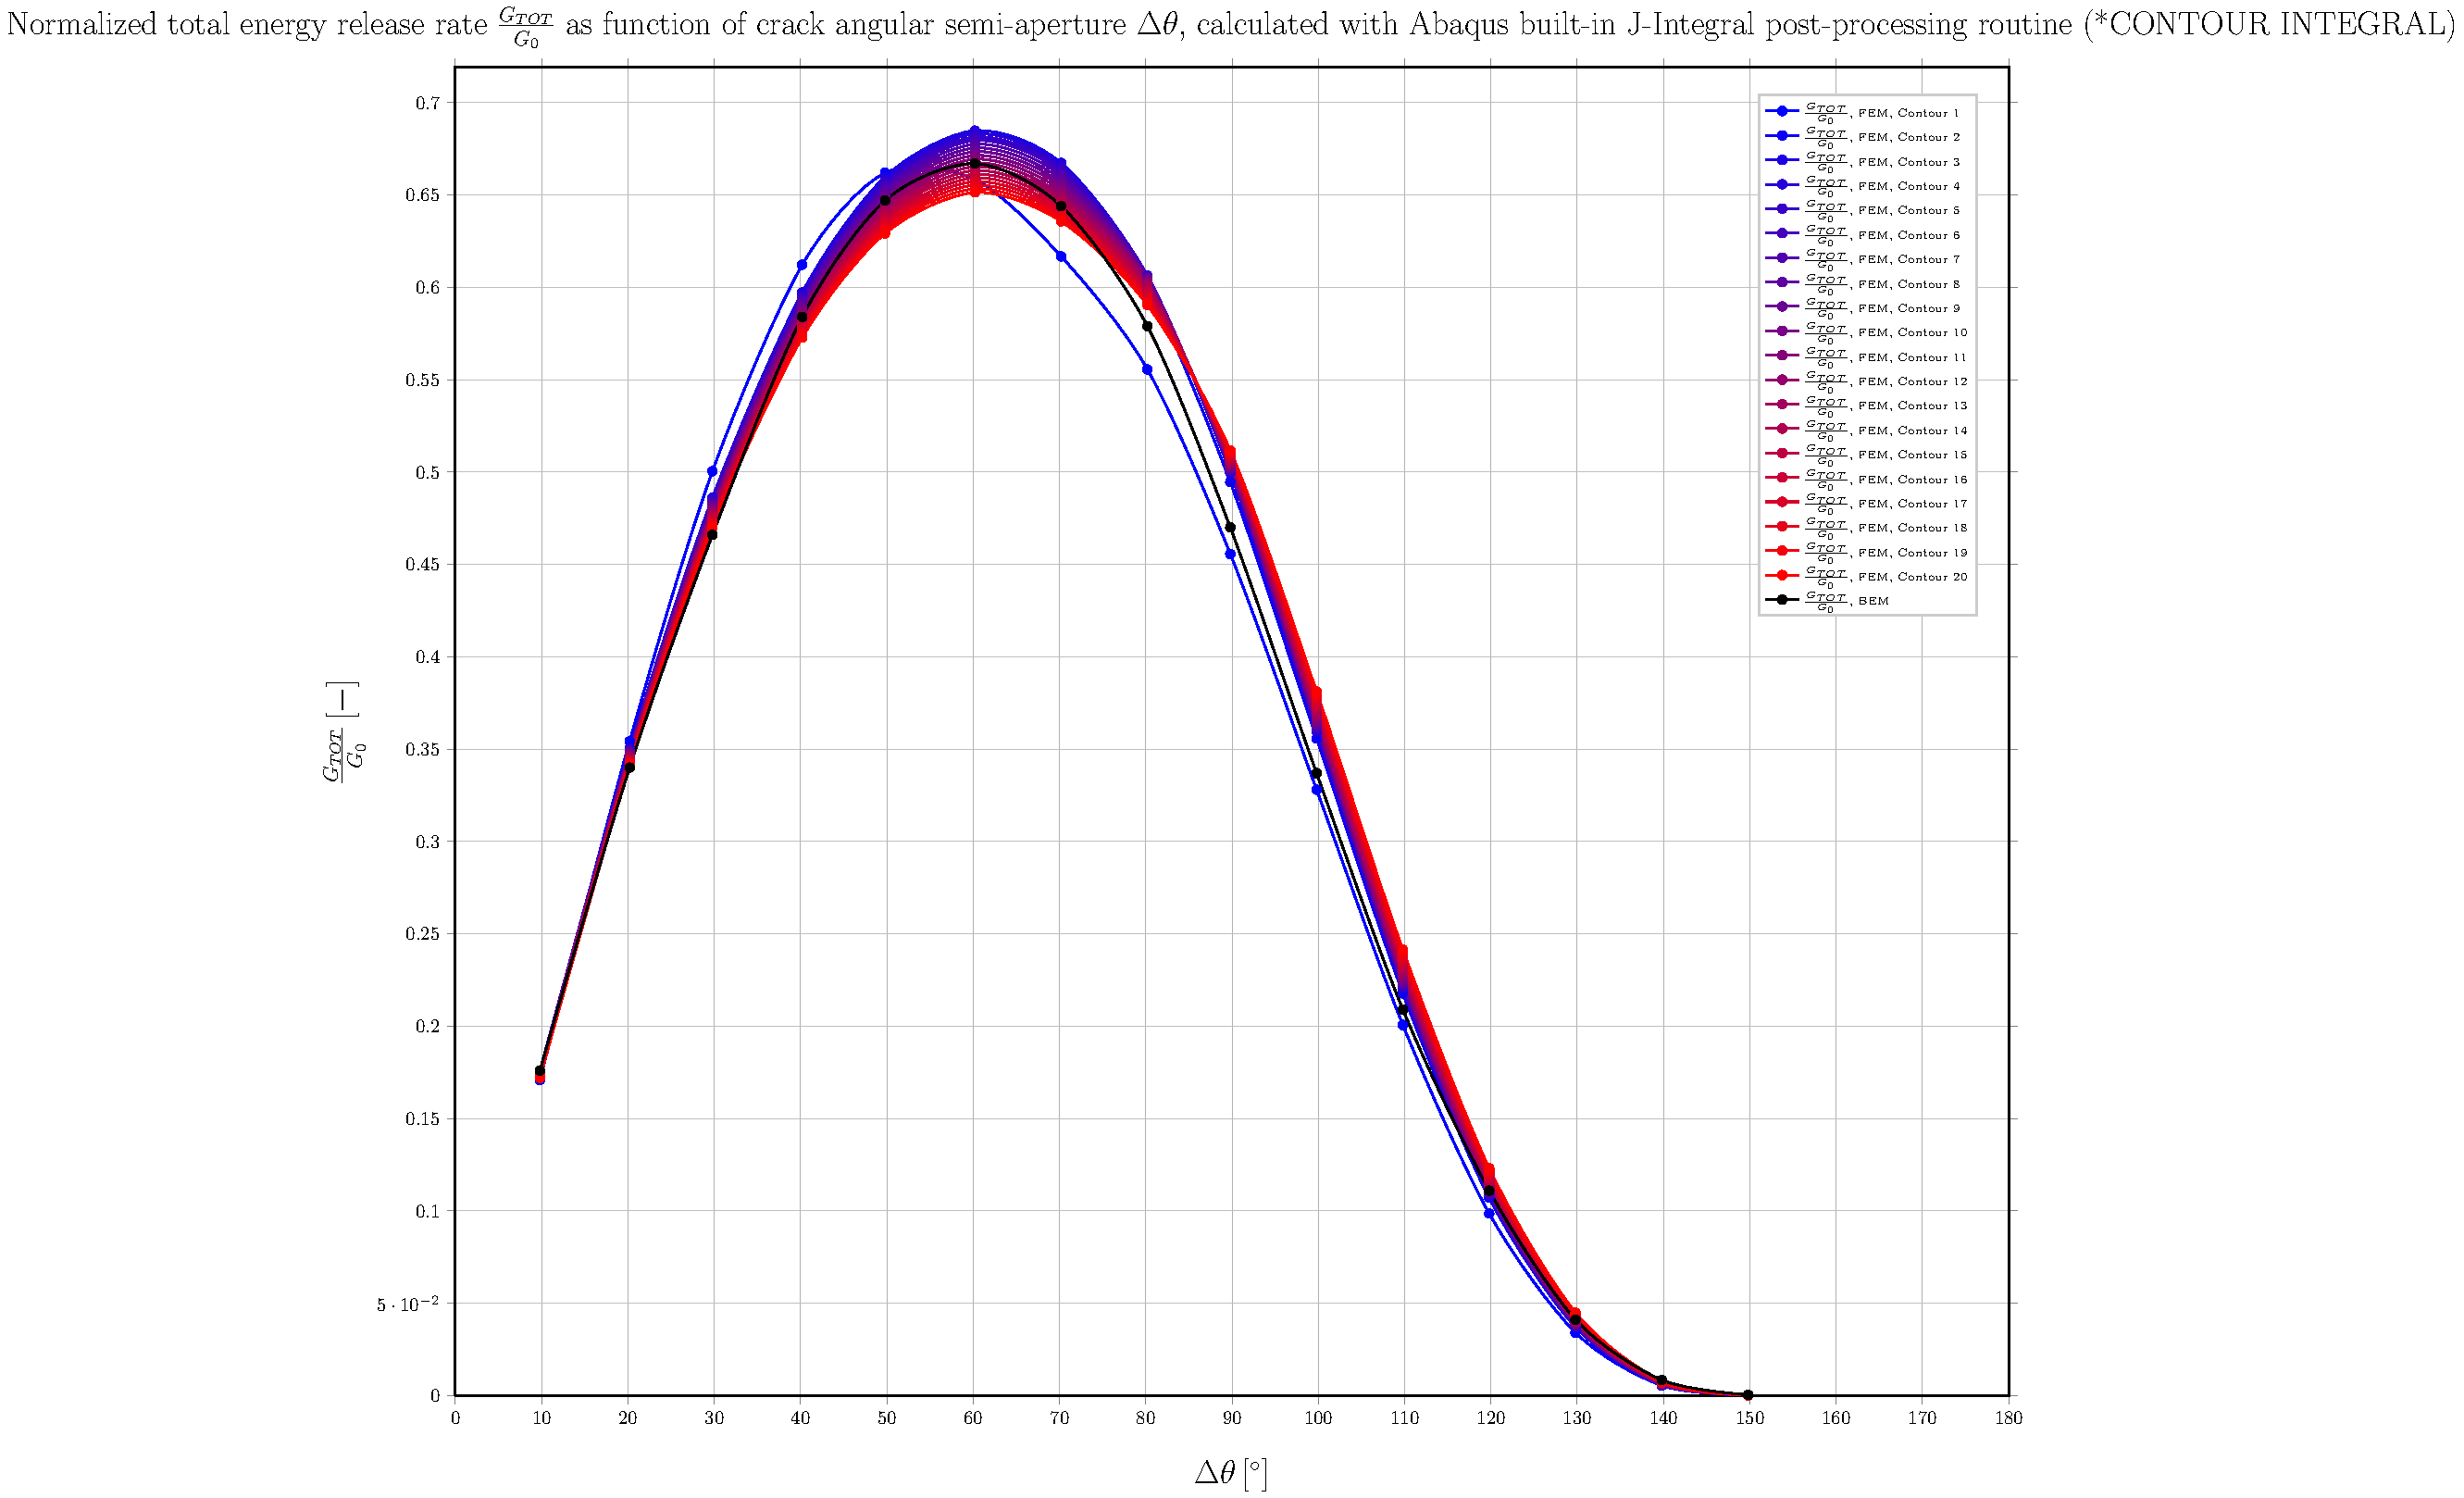
\includegraphics[height=0.7\textheight]{2017-06-23_AbqRunSummary_SingleFiberEqRfSmallStrain_J-INT_Summary.pdf}
  \caption{\scriptsize Fading from blue to red J-Integrals evaluated at contours at increasing distance from the crack tip, in black BEM results.}
  \label{fig:res1}
\end{figure}
\end{frame}

\begin{frame}
\frametitle{\small $\frac{G_{\left(\cdot\cdot\right)}}{G_{0}}$ for $V_{f}=0.001$, $\frac{L}{R_{f}}\sim28$ and $\delta=0.4^{\circ}$, small strain formulation}
\vspace{-0.5cm}
\centering
\captionsetup[figure]{font=scriptsize,labelfont=scriptsize}
\begin{figure}[!h]
\centering
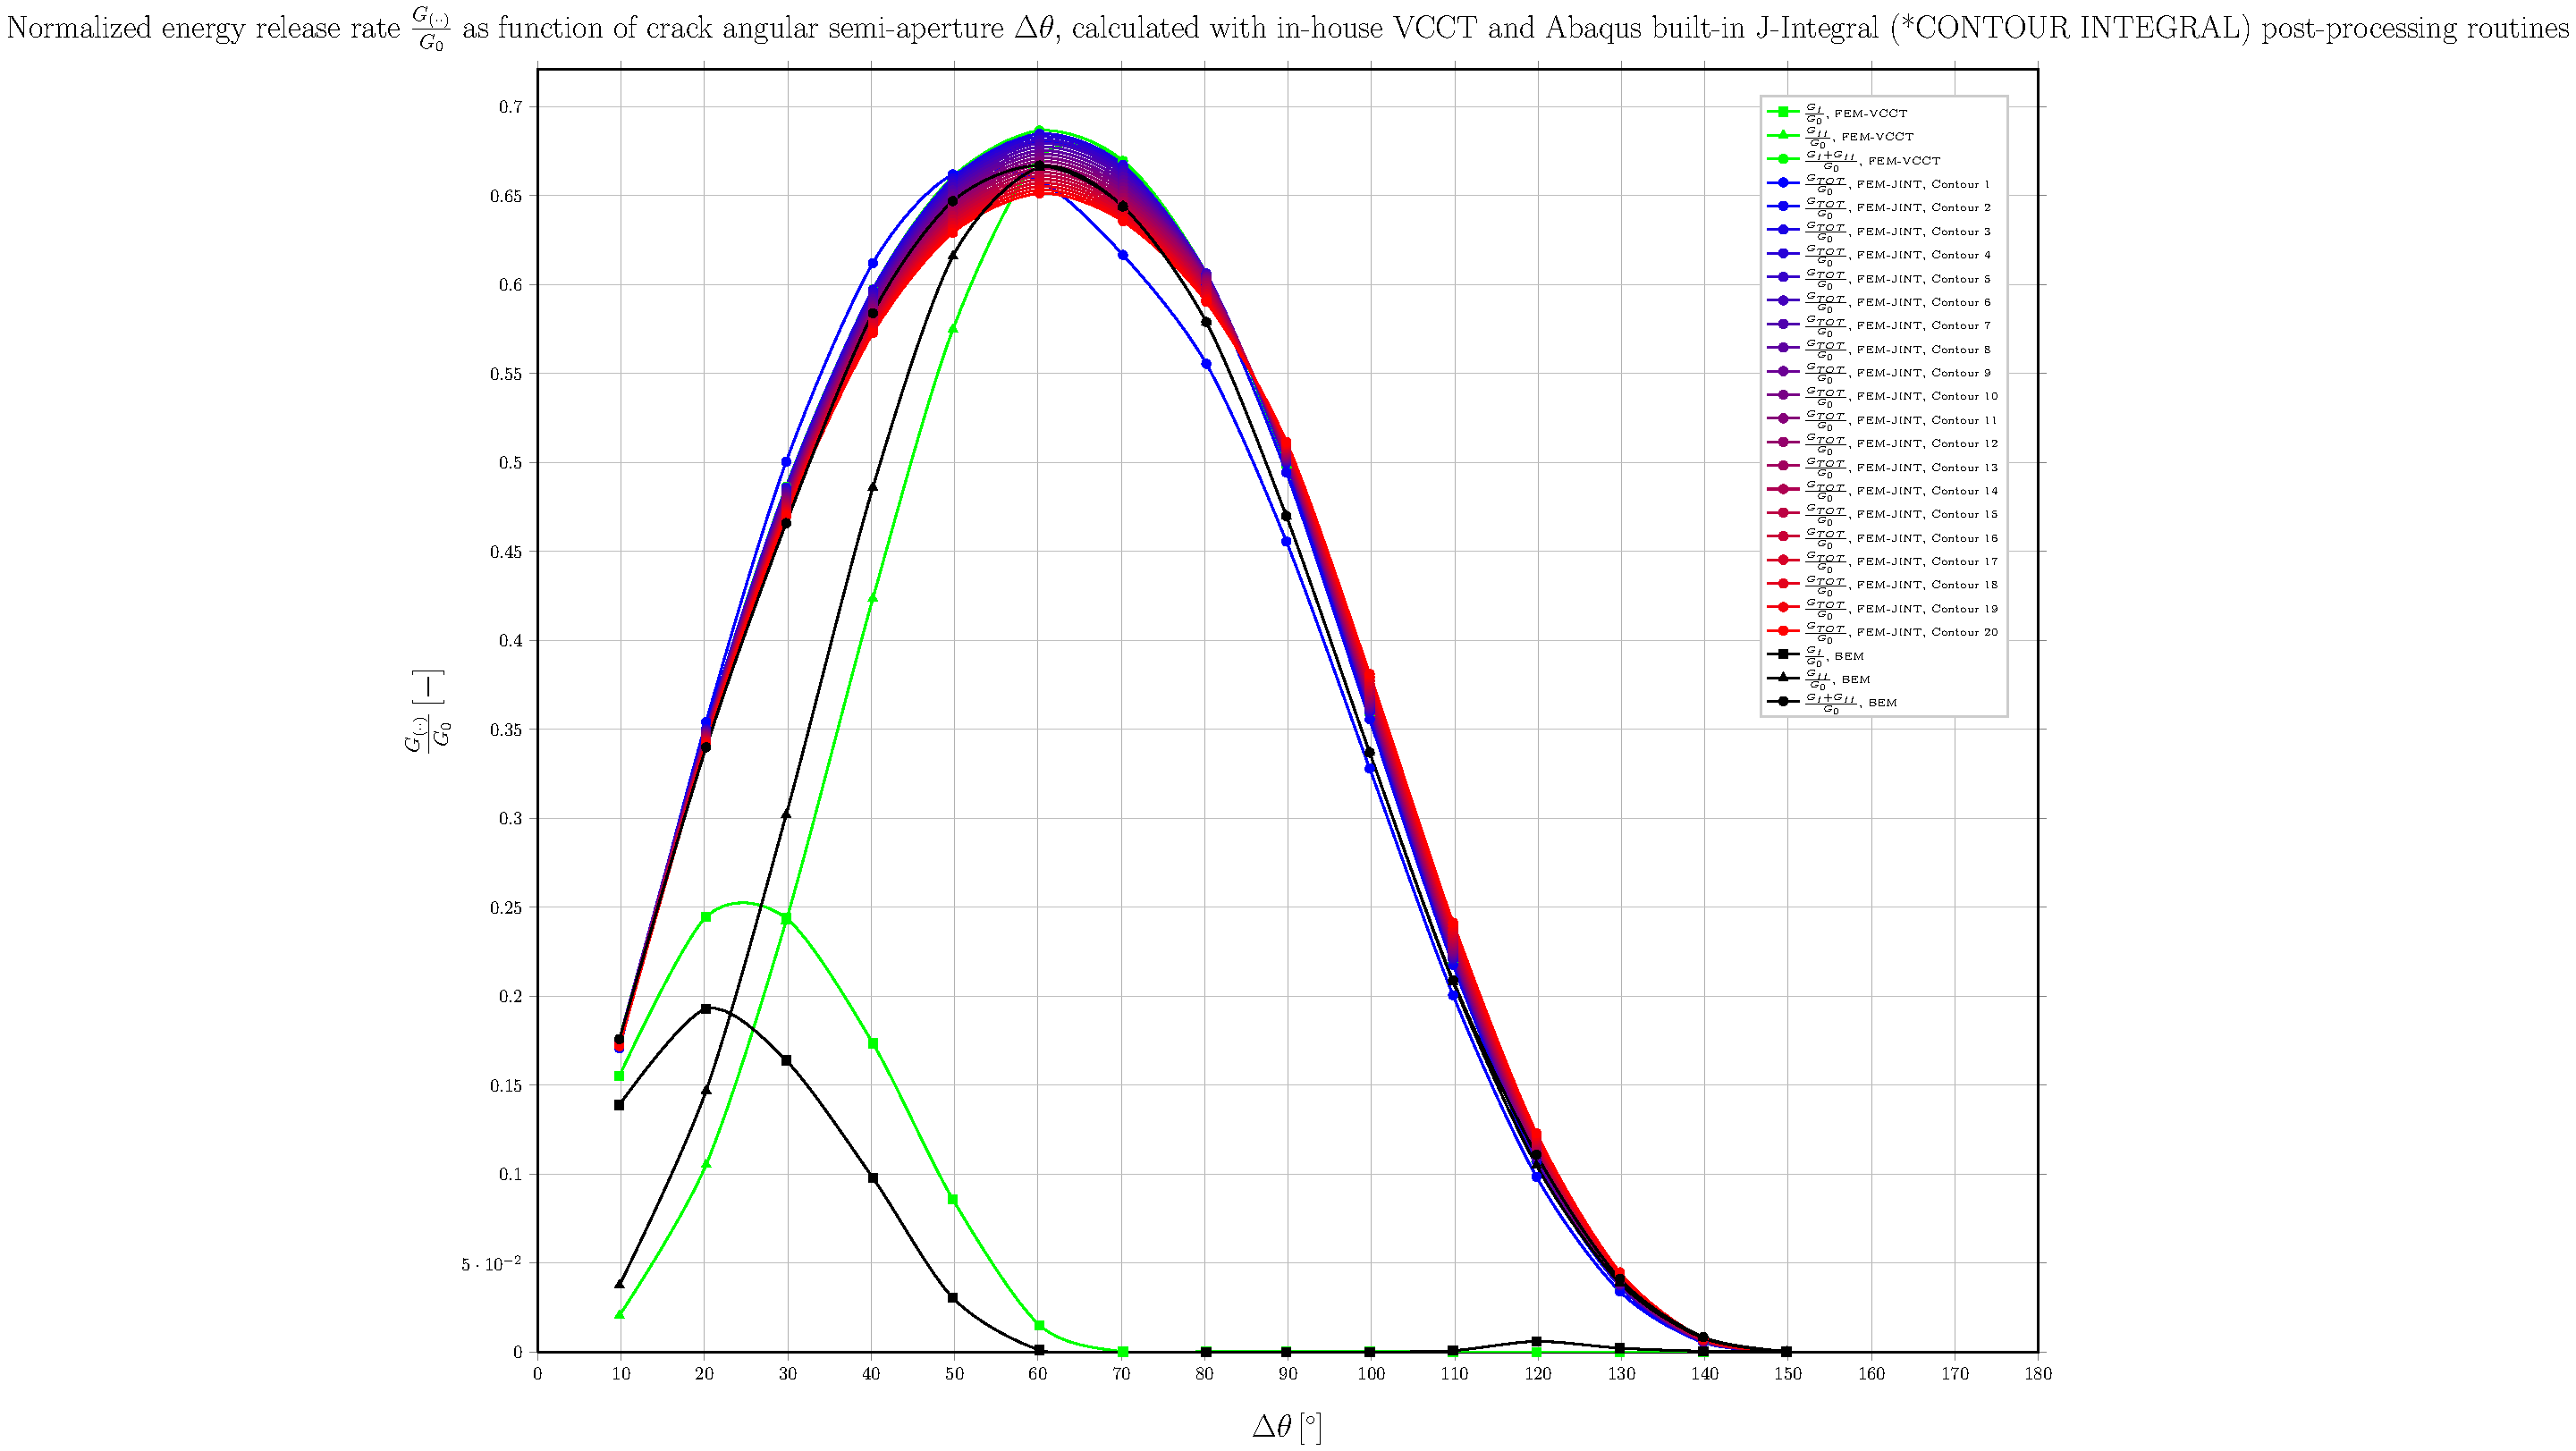
\includegraphics[height=0.7\textheight]{2017-06-23_AbqRunSummary_SingleFiberEqRfSmallStrain_VCCT-JINT_Summary.pdf}
  \caption{\scriptsize Fading from blue to red J-Integrals evaluated at contours at increasing distance from the crack tip, in green evaluation with in-house VCCT routine, in black BEM results.}
  \label{fig:res1}
\end{figure}
\end{frame}

\begin{frame}
\frametitle{\small $\frac{G_{\left(\cdot\cdot\right)}}{G_{0}}$ for $V_{f}=0.001$, $\frac{L}{R_{f}}\sim28$ and $\delta=0.4^{\circ}$, finite strain formulation}
\vspace{-0.5cm}
\centering
\captionsetup[figure]{font=scriptsize,labelfont=scriptsize}
\begin{figure}[!h]
\centering
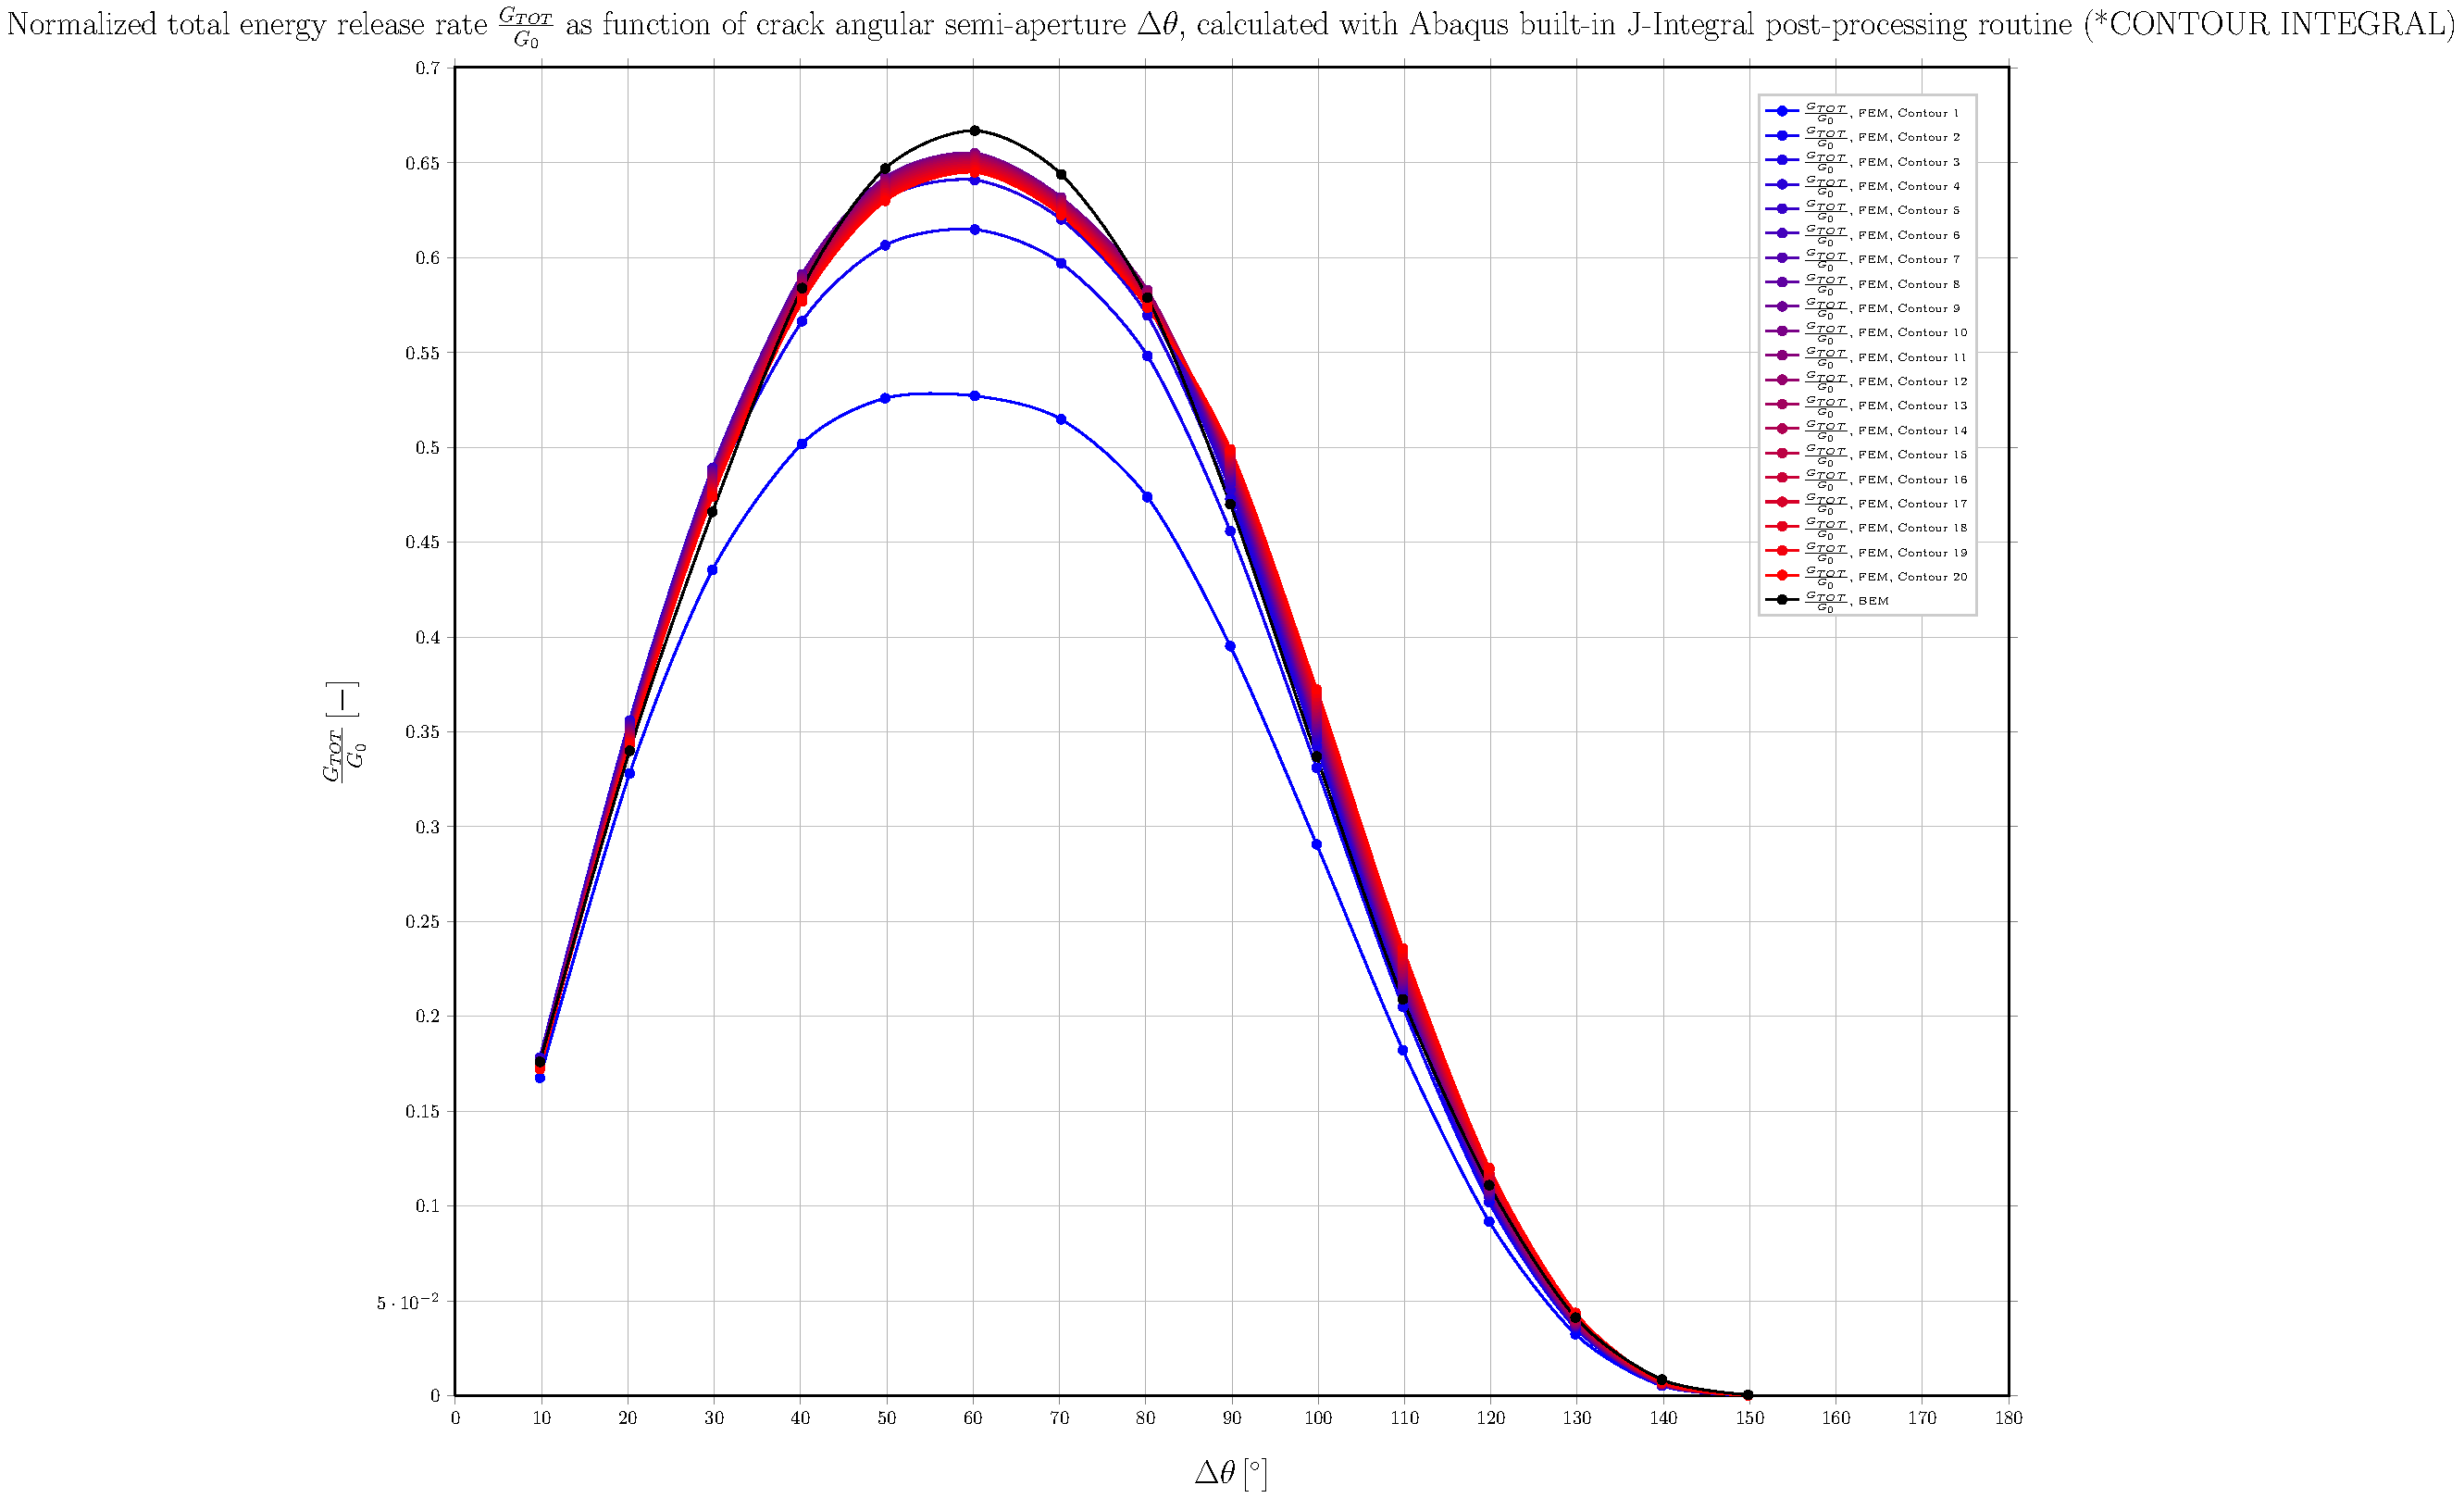
\includegraphics[height=0.7\textheight]{2017-06-23_AbqRunSummary_SingleFiberEqRfFiniteStrain_J-INT_Summary.pdf}
  \caption{\scriptsize Fading from blue to red J-Integrals evaluated at contours at increasing distance from the crack tip, in black BEM results.}
  \label{fig:res1}
\end{figure}
\end{frame}

\begin{frame}
\frametitle{\small $\frac{G_{\left(\cdot\cdot\right)}}{G_{0}}$ for $V_{f}=0.001$, $\frac{L}{R_{f}}\sim28$ and $\delta=0.4^{\circ}$, finite strain formulation}
\vspace{-0.5cm}
\centering
\captionsetup[figure]{font=scriptsize,labelfont=scriptsize}
\begin{figure}[!h]
\centering
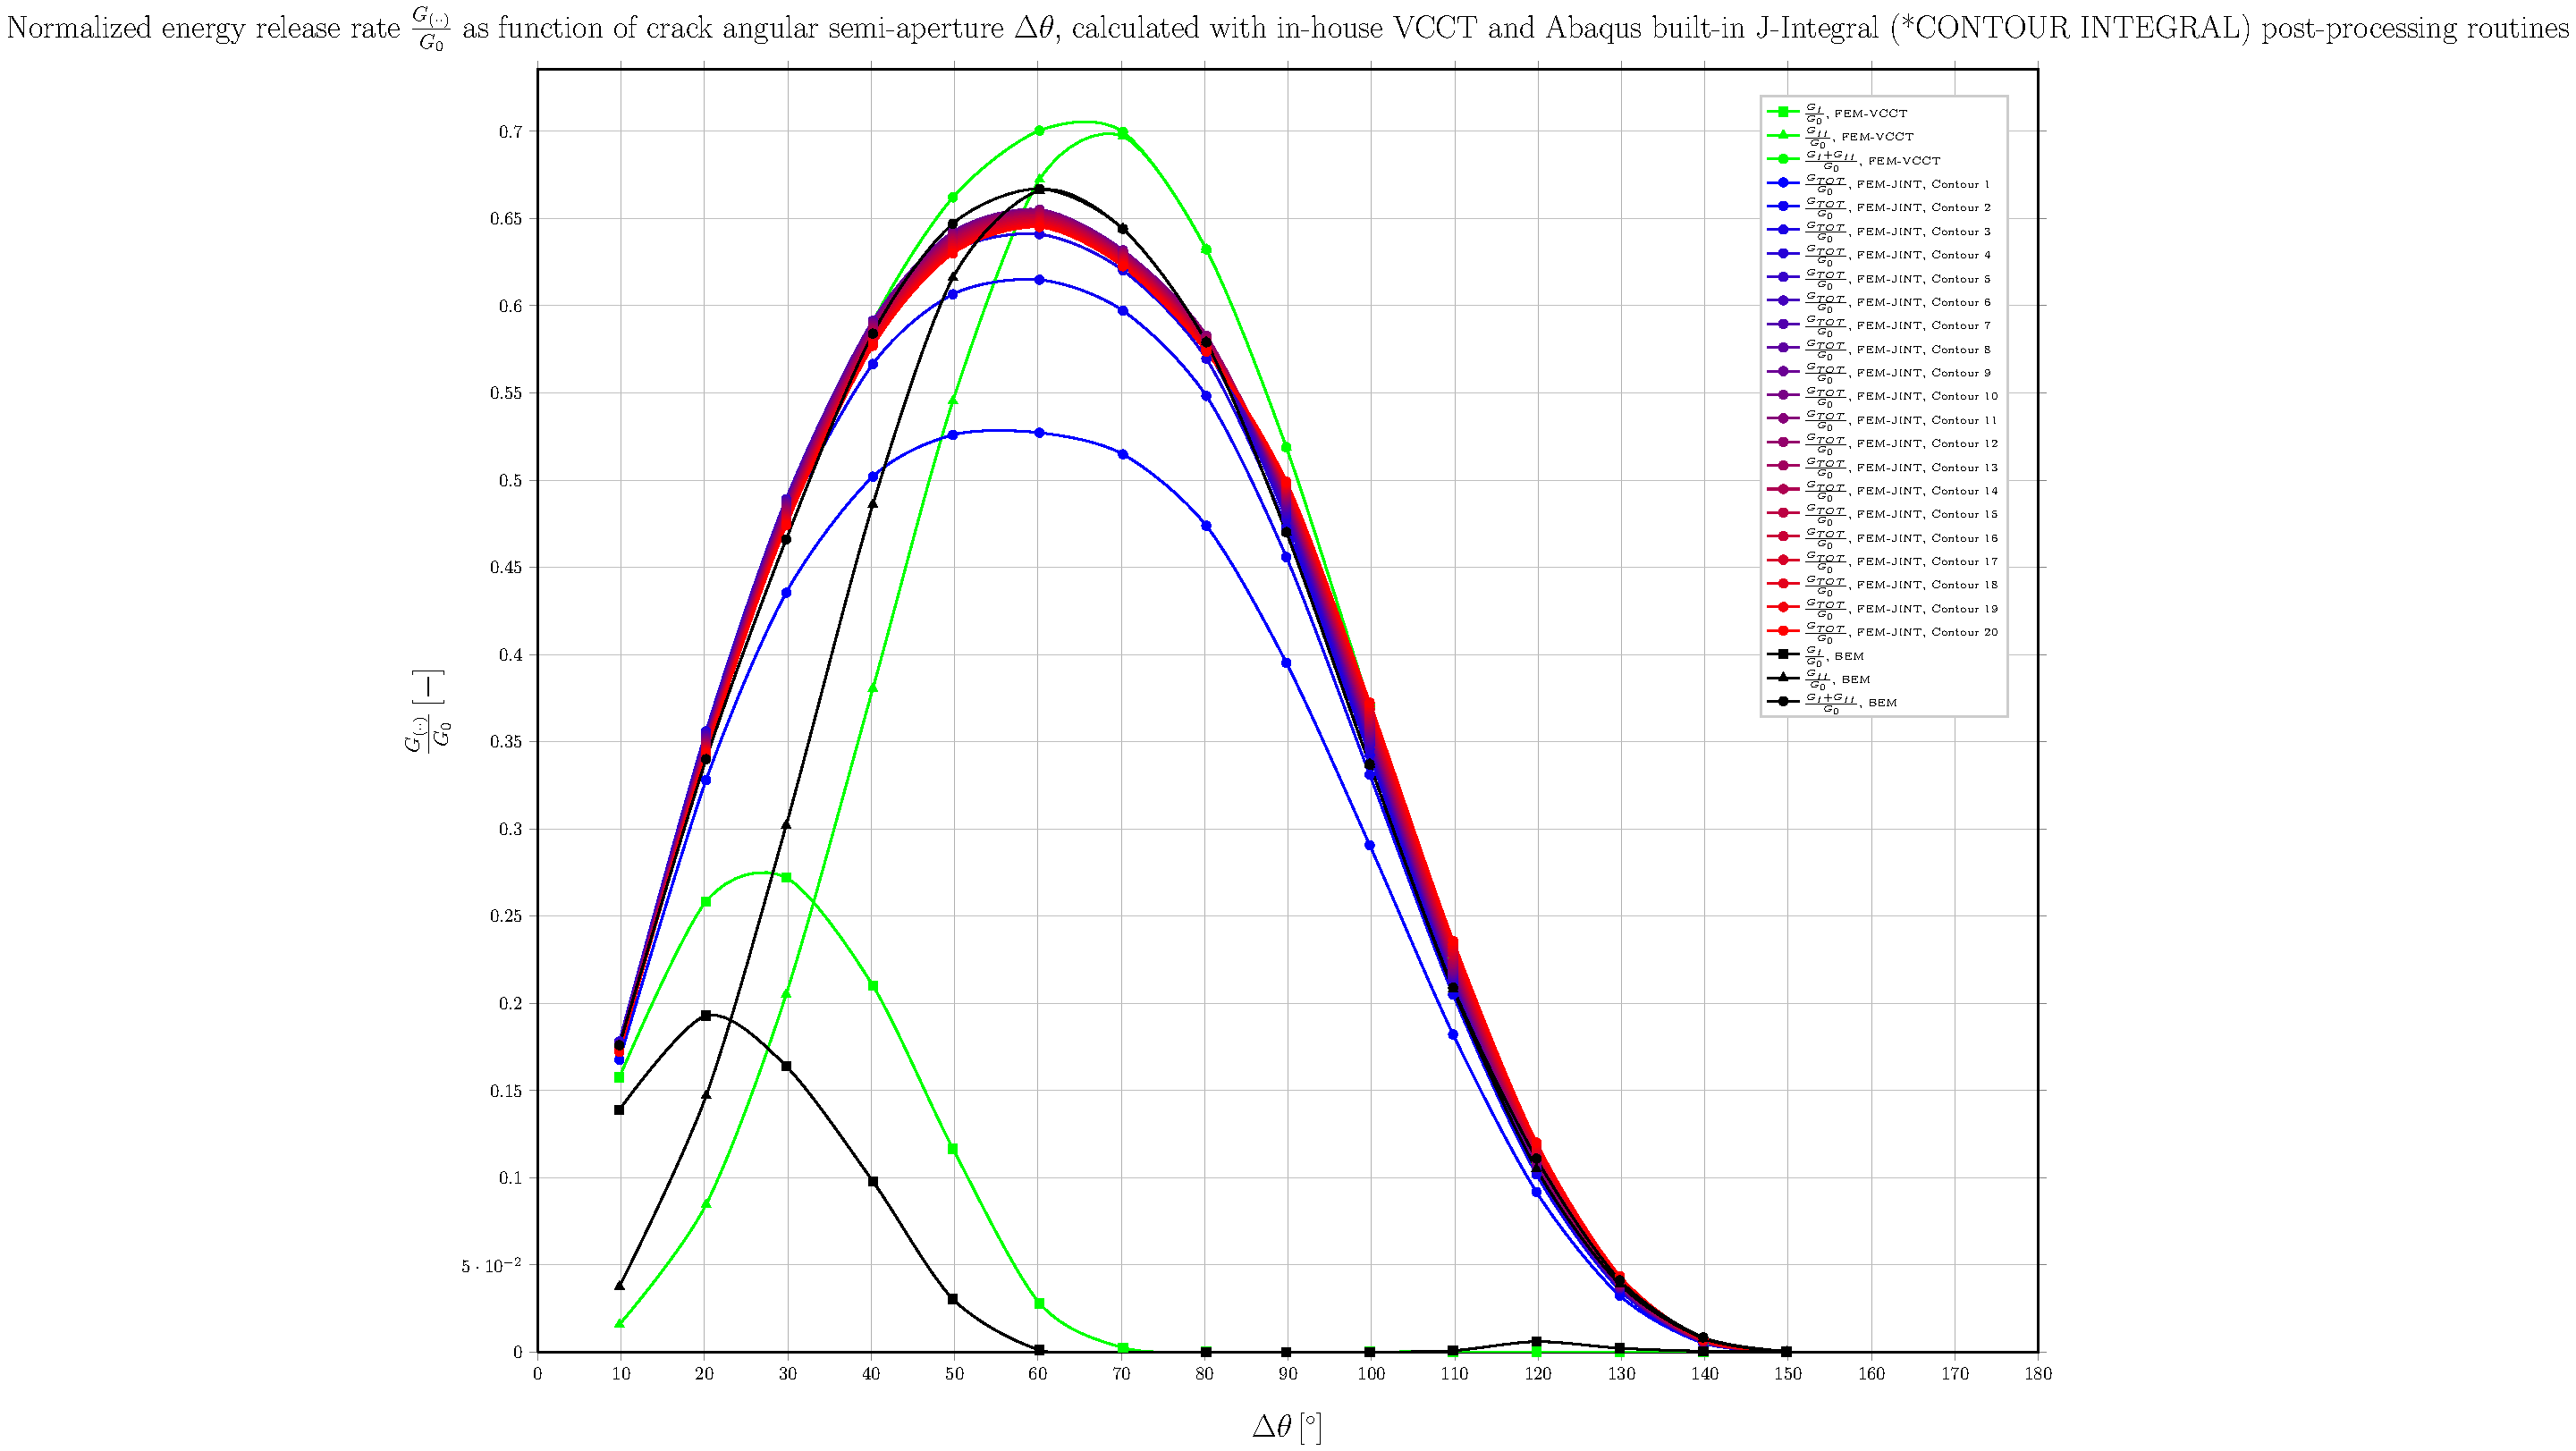
\includegraphics[height=0.7\textheight]{2017-06-23_AbqRunSummary_SingleFiberEqRfFiniteStrain_VCCT-JINT_Summary.pdf}
  \caption{\scriptsize Fading from blue to red J-Integrals evaluated at contours at increasing distance from the crack tip, in green evaluation with in-house VCCT routine, in black BEM results.}
  \label{fig:res1}
\end{figure}
\end{frame}

\begin{frame}
\frametitle{\small Conclusions}
\vspace{-0.5cm}
\centering
\begin{itemize}[label=\ding{212}]
\item For both small and finite strain formulations, J-integrals are already in good agreement with $\frac{G_{TOT}}{G_{0}}$ from BEM, i.e. no sizeable finite size effect already at $\frac{L}{R_{f}}\sim 28$
\item For both small and finite strain formulations, J-integrals correctly measure the peak value of $\frac{G_{TOT}}{G_{0}}$ at $60^{\circ}$
\item J-Integrals in small strain slightly overestimate the BEM result
\item J-integrals in small strain shows poor convergence in the range $50^{\circ}-80^{\circ}$
\item J-Integrals in finite strain slightly underestimate the BEM result
\item J-integrals in finite strain shows very good convergence in all the range $10^{\circ}-150^{\circ}$
\end{itemize}
\end{frame}

\begin{frame}
\frametitle{\small Conclusions}
\vspace{-0.5cm}
\centering
\begin{itemize}[label=\ding{212}]
\item $\frac{G_{TOT}}{G_{0}}$ is correctly calculated by the VCCT in small strain, in good agreement with BEM results
\item The peak value of $\frac{G_{TOT}}{G_{0}}$ is correctly calculated by the VCCT in small strain, at $60^{\circ}$
\item $\frac{G_{TOT}}{G_{0}}$ is wrongly calculated by the VCCT in finite strain, with a peak at $65^{\circ}-70^{\circ}$
\item Small strain VCCT shows better results than finite strain VCCT
\item Mode ratio is still not correct, i.e. probably finite size effect
\end{itemize}
\end{frame}

\begin{frame}
\frametitle{\small Observations \& Questions}
\vspace{-0.45cm}
\centering
\begin{itemize}[label=\ding{212}]
\item J-Integral is a far-field technique, using stresses, strain and displacements far from the crack tip; convergence is in fact far from crack tip (at least 10 contours, i.e. 10 ring of elements)
\item VCCT is a local technique, using forces and displacements at the crack tip
\item The difference between small and finite strain results rests mainly in the displacements
\item Previously, we observed that changing the formulation of the bonded interface, all other parameters equal, the result doesn't change
\item All the convergence problem reduces to the correct evaluation of displacements of debonded surfaces close to the crack tip
\item Displacements of debonded surfaces close to the crack tip are influenced by RVE size
\end{itemize}
\end{frame}

\begin{frame}
\frametitle{\small Observations \& Questions}
\vspace{-0.25cm}
\centering
\begin{itemize}[label=\ding{212}]
\item Small strain shows (correctly) better results than finite strain formulation with respect to infinite reference values
\item However, Abaqus documentation suggests that, if contact between surfaces is present in the model, finite strain formulation (nonlinear geometry) should be used
\item For finite sizes of RVE, which formulation should be chosen?
\end{itemize}
\end{frame}

\section{Elements's aspect ratio}

\begin{frame}
\frametitle{\small $\frac{G_{\left(\cdot\cdot\right)}}{G_{0}}$ for  $Vf_{f}=0.000079$, $\frac{L}{R_{f}}\sim100$ and $\delta=1.0^{\circ}$, small strain formulation}
\vspace{-0.5cm}
\centering
\captionsetup[figure]{font=scriptsize,labelfont=scriptsize}
\begin{figure}[!h]
\centering
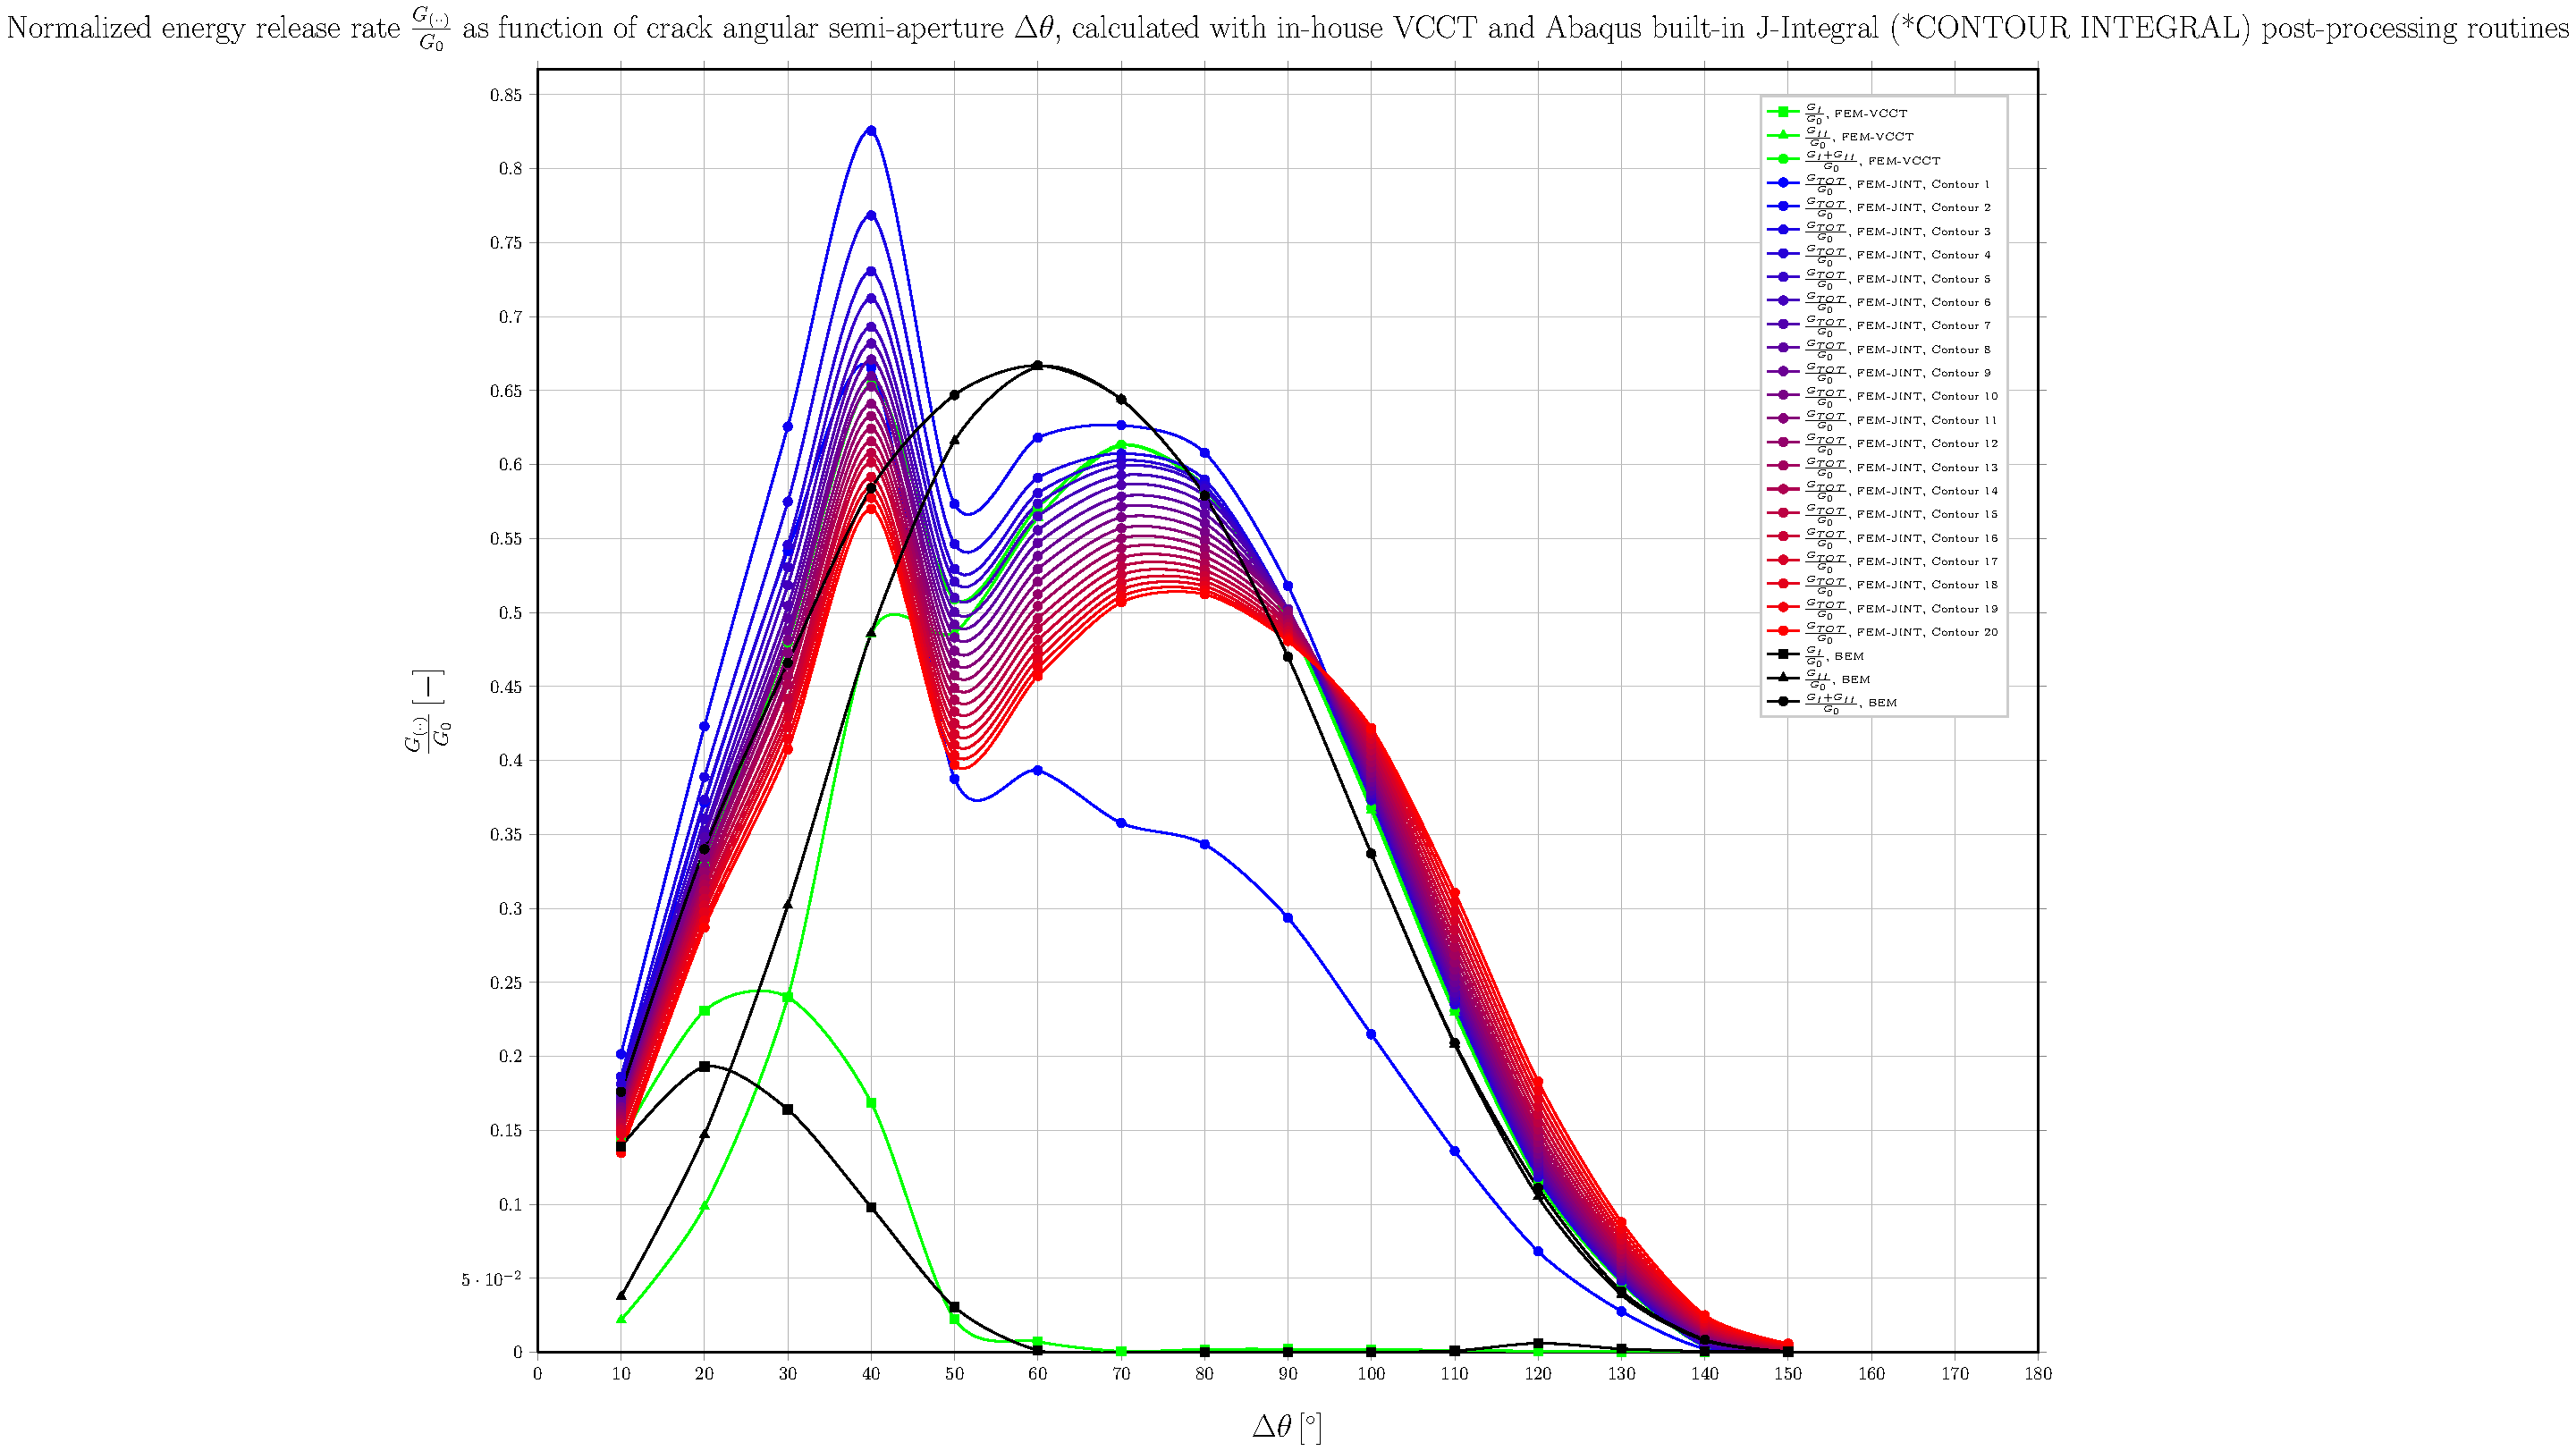
\includegraphics[height=0.7\textheight]{2017-06-16_AbqRunSummary_SingleFiberEqRfSmallStrain-D1-0_VCCT-JINT_Summary.pdf}
  \caption{\scriptsize Fading from blue to red J-Integrals evaluated at contours at increasing distance from the crack tip, in green evaluation with in-house VCCT routine, in black BEM results.}
  \label{fig:res1}
\end{figure}
\end{frame}

\begin{frame}
\frametitle{\small $\frac{G_{\left(\cdot\cdot\right)}}{G_{0}}$ for  $Vf_{f}=0.000079$, $\frac{L}{R_{f}}\sim100$ and $\delta=0.4^{\circ}$, small strain formulation}
\vspace{-0.5cm}
\centering
\captionsetup[figure]{font=scriptsize,labelfont=scriptsize}
\begin{figure}[!h]
\centering
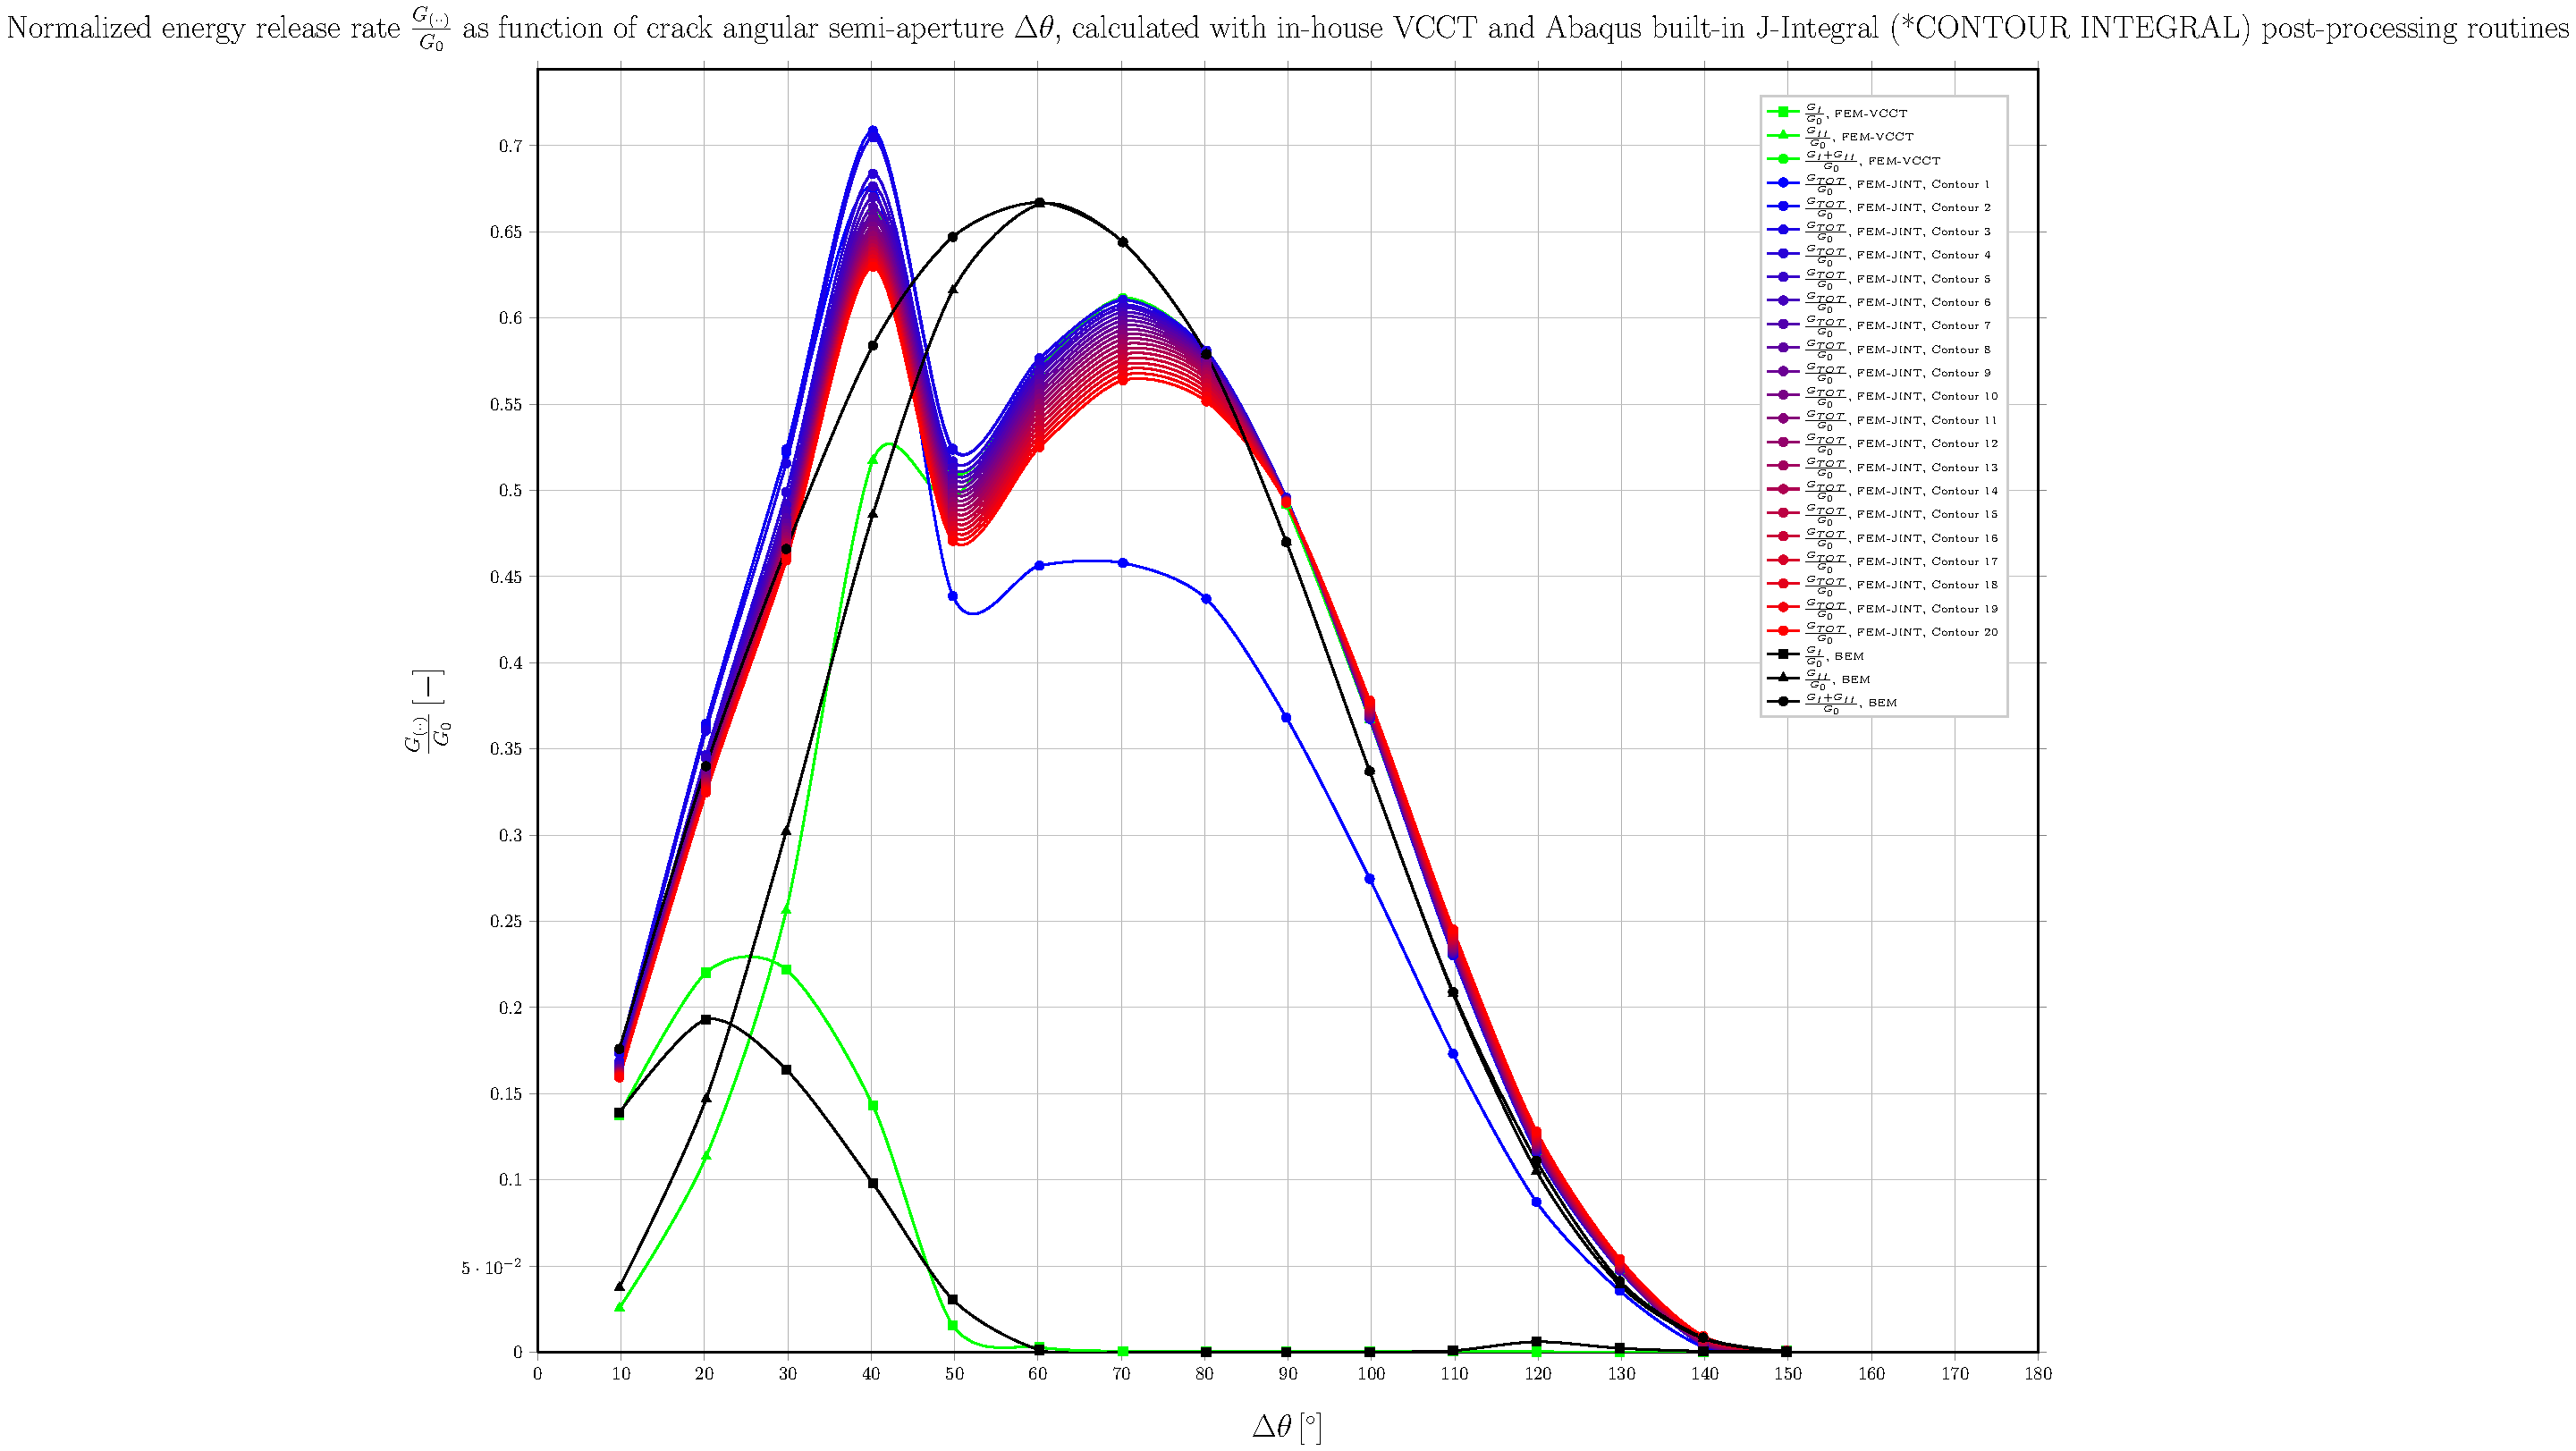
\includegraphics[height=0.7\textheight]{2017-06-16_AbqRunSummary_SingleFiberEqRfSmallStrain-D0-4_VCCT-JINT_Summary.pdf}
  \caption{\scriptsize Fading from blue to red J-Integrals evaluated at contours at increasing distance from the crack tip, in green evaluation with in-house VCCT routine, in black BEM results.}
  \label{fig:res1}
\end{figure}
\end{frame}

\begin{frame}
\frametitle{\small Conclusions}
\vspace{-0.5cm}
\centering
\begin{itemize}[label=\ding{212}]
\item Elements' aspect ratio (maximum side length/minimum side length) was very high in the exterior part of the matrix in this set of simulations
\item Spurious stresses adn deformations were created at $45^{\circ},135^{\circ},225^{\circ},315^{\circ}$
\item Results are badly affected by this in the range  $40^{\circ} - 70^{\circ}$ with a marked oscillation between $40^{\circ} - 50^{\circ}$
\item Elements' aspect ratio in the matrix is more important than the elements' size at the fiber/matrix interface
\item Program has already been changed to receive aspect ratios as input instead of number of elements
\item Results from previous sections were calculated with meshes with controlled aspect ratios
\end{itemize}
\end{frame}

\section{Next steps}

\begin{frame}
\frametitle{\small Next steps}
\vspace{-0.5cm}
\centering
\begin{itemize}[label=\ding{212}]
\item Simulations for $Vf_{f}=7.9\cdot 10^{-5}$, $\frac{L}{R_{f}}\sim 100$ for different $\delta$ (mesh size) for both finite and small strain: already running, results during next week
\item Simulations over $Vf_{f}$ for fixed $\Delta\theta$ and $\delta$ to find the value of $Vf_{f}$ for which the model can be considered infinite by measuring $\sigma_{0}$ and $G_{0}$: starting beginning next week ($\sim$Monday)
\item Simulations over elements' aspect ratio for fixed size and $Vf_{f}$ to measure its effect on the solution: starting mid next week ($\sim$Wednesday)
\end{itemize}
\end{frame}

%\section{Appendices \& References}
%
%\subsection{Appendices}
%
%
%%\end{frame}
%
%\subsection{References}
%
%\begin{frame}[allowframebreaks]
%  \frametitle{References}
%    
%  \begin{thebibliography}{10}
%    
%%  \beamertemplatebookbibitems
%%  % Start with overview books.
%%
%%  \bibitem{Author1990}
%%    A.~Author.
%%    \newblock {\em Handbook of Everything}.
%%    \newblock Some Press, 1990.
% 
%    
%  \beamertemplatearticlebibitems
%  % Followed by interesting articles. Keep the list short. 
%
%\bibitem{DonaldL.Flaggs1982}
%Donald L. Flaggs, Murat H. Kural;
%\newblock {\em Experimental Determination of the In Situ Transverse Lamina Strength in Graphite/Epoxy Laminates.}
%\newblock Journal of Composite Materials, vol. 16, n. 2, 1982.
%
%\bibitem{Parvizi1978}
%Parvizi A., Bailey J.E;
%\newblock {\em On multiple transverse cracking in glass fibre epoxy cross-ply laminates.}
%\newblock Journal of Materials Science, 1978; 13:2131-2136.
%
%\bibitem{herraez2015}
%Miguel Herr\'aez, Diego Mora, Fernando Naya, Claudio S. Lopes, Carlos Gonz\'alez, Javier LLorca;
%\newblock {\em Transverse cracking of cross-ply laminates: A computational micromechanics perspective.}
%\newblock Composites Science and Technology, 2015; 110:196-204.
%
%\bibitem{Canal2012}
%Luis Pablo Canal, Carlos Gonz\'alez, Javier Segurado, Javier LLorca;
%\newblock {\em Intraply fracture of fiber-reinforced composites: Microscopic mechanisms and modeling.}
%\newblock Composites Science and Technology, 2012; 72(11):1223-1232.
%
%\bibitem{StephenW.Tsai2005}
%Stephen W. Tsai;
%\newblock {\em Thin ply composites.}
%\newblock JEC Magazine 18, 2005.
%
%
%\bibitem{ZnedekP.Bazant2002}
%Znedek P. Bazant;
%\newblock {\em Size Effect Theory and its Application to Fracture of Fiber Composites and Sandwich Plates.} 
%\newblock in Continuum Damage Mechanics of Materials and Structures, eds. O. Allix and F. Hild, 2002.
%
%
%\bibitem{RobinAmacherWayneSmithClemensDransfeldJohnBotsis2014}
%Robin Amacher, Wayne Smith, Clemens Dransfeld, John Botsis, Jo\"el Cugnoni;
%\newblock {\em Thin Ply: from Size-Effect Characterization to Real Life Design}
%\newblock CAMX 2014, 2014
%
%\bibitem{RalfCuntze}
%Ralf Cuntze;
%\newblock {\em The  World-Wide-Failure-Exercises -I  and - II for UD-materials.}
%
%
%\bibitem{Pinho}
%Pinho, S. T. and Pimenta, S.;
%\newblock {\em Size Effects on the Strength and Toughness of Fibre-Reinforced Composites.}
%
%\bibitem{PedroP.CamanhoCarlosG.DavilaSilvestreT.PinhoLorenzoIannucci2006}
%Pedro P. Camanho, Carlos G. D\'avila, Silvestre T. Pinho, Lorenzo Iannucci, Paul Robinson;
%\newblock {\em Prediction of in situ strengths and matrix cracking in composites under transverse tension and in-plane shear.}
%\newblock Composites Part A: Applied Science and Manufacturing, vol. 37, n. 2, 2006.
%
%\bibitem{P.P.CamanhoP.Maimi2007}
%P.P. Camanho, P. Maim\'i, C.G. D\'avila;
%\newblock {\em Prediction of size effects in notched laminates using continuum damage mechanics.}
%\newblock Composites Science and Technology, vol. 67, n. 13, 2007.
%
%\bibitem{Nairn1992}
%J. A. Nairn;
%\newblock {\em The Initiation and Growth of Delaminations Induced by Matrix Microcracks in Laminated Composites.}
%\newblock International Journal of Fracture, vol. 57, 1992.
%
%\bibitem{JoelCugnoniRobinAmacher2013}
%Joel Cugnoni , Robin Amacher, John Botsis;
%\newblock {\em Thin ply technology advantages. An overview of the TPT-TECA project.}
%\newblock 2014.
%
%
%  \end{thebibliography}
%\end{frame}

\begin{frame}[plain]
\frametitle{}
\end{frame}

\end{document}

